%%%%%%%%%%%%%%%%%%%%%%%%%%%%%%%%%
% 6CCS3PRJ Final Year Individual Project Report
% luke.day@kcl.ac.uk
%%%%%%%%%%%%%%%%%%%%%%%%%%%%%%%%%
\documentclass[11pt]{informatics-report}
\usepackage{xcolor}
\usepackage{natbib} %References
\usepackage{graphicx}

%%%%%%%%%%%%%%%%%%%%%%%%%%%%%%%%%
% Front Matter - project title, name, supervisor name and date
%%%%%%%%%%%%%%%%%%%%%%%%%%%%%%%%%
\title{Automated Grading of SQL Tasks to Improve Student Learning}
\author{Vlad Stoica}
\studentID{1531350}
\supervisor{Criado Pacheco, Natalia}

\date{\today}

\abstractFile{FrontMatter/abstract.tex}
\ackFile{FrontMatter/acknowledgements.tex} %Remove line if you do not want acknowledgements

\begin{document}
\createFrontMatter
\onehalfspacing
\tableofcontents
\doublespacing

\definecolor{code-background}{gray}{0.97}

%%%%%%%%%%%%%%%%%%%%%%%%%%%%%%%%%
% Report Content
%%%%%%%%%%%%%%%%%%%%%%%%%%%%%%%%%
% You can write each chapter directly here or in a separate .tex file and use the include command.

\chapter{Introduction} \label{ch:introduction}
\section{Project motivations}
With the technological advancements of the 21st century, acquiring and interpreting
data has become essential for almost all areas of the economy. The \cite{ec:big_data} argues that ''good use of data is at
the centre of the future knowledge economy''.
Furthermore, the \cite{gov:big_data} also believes ``data can truly be a catalyst for a society, an economy, a country that works for everyone''. With this in mind, more and more companies acknowledge the importance of analyzing data and employing data analysts in their companies. It is estimated the US needs over 140.000 workers with ``data analytical expertise'' \citep{Lohr2012}.

One of the most popular data sources in any company is usually represented by the main database, which stores various data. 6 out of 10 most popular databases are Relation Database Management Systems (RDBMS) \citep{db_engine:statistics}.
Accessing data in an RDBMS is done through \textit{Standard Query Language}
(SQL); therefore, course providers recognize the need to introduce programs that teach their students how to use SQL, in order to make them more employable.

Nowadays, SQL is being taught to almost all students in a Computer Science
degree. This project will explore how assessing student's SQL
assignments can be automated and become more accurate. There have been many attempts at improving this process made by various scholars, such as \cite{literature:activesql}, \cite{literature:assesql},
\cite{literature:sqlify}, \cite{literature:xdata}. This project builds on the existing work of these scholars, especially that of \cite{literature:xdata} in their project - \textbf{XData}.

\section{SQL assignments} \label{ch:introduction:assignments}

An important part of teaching any module is represented by assessments. They motivate the students to learn throughout the year and often promote deep learning, allowing students to get a better understanding of the material \citep{literature:assement}.

Another important role played by assessments throughout the year is the guidance offered to students based on the feedback provided on their earlier work \citep{literature:assement}. According to \cite{literature:assement}, the better the feedback provided, the greater the likelihood of students improving their performance. Effective feedback can help students understand what mistakes they make and also provides information about how to fix them \citep{literature:assement}.

With all these advantages in mind, it is obvious SQL assignments are essential to success. SQL assessments usually consist of the following components:
\begin{itemize}
    \item A SQL table schema provided by the teacher. The schema includes
    the structure of the database tables and any relations between them;
    \item A SQL query that inserts the initial data in the database;
    \item A description of the assessment;
    \item A correct SQL query solution for the
    assignment.
\end{itemize}

The assessment requires a SQL query from the student that fits the requirements mentioned in the description of the problem. The query should return the same results as the query provided by the teacher. In general, these assignments are marked manually by Instructors or Teaching Assistants (TAs) \citep{literature:xdata}. Marking SQL manually is a very time consuming process which often leads to a very long time between the submission of work and students receiving feedback on the assignment. If the time between those two milestones is too long, it is often the case students will not be able to acknowledge or understand their mistakes in time for future assignments. This represents a crucial problem when considering the importance of learning from mistakes or difficulties \citep{literature:assement}.

As previously mentioned, attempts at automating this process have been made. Various tools have been built, which are presented in more detail in the next chapter. However, most of these tools are only deployed in the courses taught by the authors, with no popular tool widely used in academia. Automating the assessment process brings multiple benefits:
\begin{itemize}
    \item It can give more time for TAs and teachers to focus on better helping students, rather than spending a great amount of time grading assignments.
    \item It opens the possibility of introducing more assignments throughout the course, which would further enhance students' learning process. Although it is generally better to provide less assignments which are more meaningful due to time constraints. \citep{literature:assement}, automating this process means time constraints are no longer relevant.
    \item It can provide instant feedback on assignments. As mentioned earlier, feedback can help students improve throughout the course. In addition, instant feedback opens the possibility for a new type of assignment, one which is not part of the grade, but instead allows the student to practice their skills. This "practice" mode has been used by multiple commercial tools, allowing anyone to learn SQL by practicing and receiving instant feedback. The level of feedback is essential however, as a simple correct / incorrect might not be of very much help.
\end{itemize}


\section{Project aims} \label{ch:introduction:sec:project_aims}

The main aim of this project is to provide a tool that can automate grading of students' tasks in SQL. In particular, the tool will produce individual grades and feedback for students who have completed a SQL assignment. This tool will be able to provide hints or suggestions when students make errors (for instance, suggest if an user is missing a table in their query, or if they are selecting the wrong columns).

The project will also produce a web application where teachers will be able to create assignments for students, and where students will be able to provide solutions to them. The student will see instant feedback on their work with hints provided if they make mistakes. In addition, teachers will be able to see a breakdown of students' assignments based on the components of a query.

\section{Report structure}

This report will begin with an overview of the available commercial applications for grading SQL, as well as a literature review, looking at existing work done on automating assessing SQL in academia.

The next chapter will present the requirements of the applications, which will be separated in two parts: the requirements for the web application, and the requirements for the grading algorithm. The chapter will then continue with the specifications section, which will first discuss the selection of programming language and the reason for choosing it, then present the development process, and finally present individual specifications for each requirement.

The fourth chapter of the report will be the design one. The chapter will present the overall system architecture before moving on to the design of each component of the project (the web application and the library), and concluding with a section about the integration between the two components.

The following chapter will discuss the implementation and testing of the application. This chapter will cover the most important and relevant implementation details from both the web application and the library. The main focus will be on the grading algorithm as this is the core output of the project. The chapter will end with a discussion of the testing mechanisms used to ensure the software runs according to the requirements.

The sixth chapter will present how the project was evaluated. We will look at three important indicators: how the scope was attained, how the project compares with existing tools, and empirically evaluate the project using exercises from various data sources.

The next chapter will look at legal, social, ethical and professional issues associated with the project. The chapter will begin with a section that looks at the issues related to the use of automated grading and its implications. The next section will present how the project follows both BCS's Code of Conduct and BCS's Code of Good Practice, concluding with a section discussing the use of open-source libraries.

The 8th and last chapter of the main body of the report will present the conclusion of the project. The chapter will present an overview of the work achieved, its limitations and suggested future work.
\chapter{Background}

\section{Commercial tools for learning SQL} \label{ch:lit:sec:tutor:comercial}

As mentioned before, SQL is one of the most in-demand skills
nowadays. This led to the appearence of multiple commercial 
applications that assess SQL. Most of them are used for helping people
learn SQL.

\subsubsection{HackerRank}
HackerRank is one of the most popular tools in the tech recruitment world,
and also allows SQL questions. The application fits most, but not all of our
needs. First of all, the application is closed-source therefore it cannot be extended. Second of all, the application does not allow regular
users to create new challenges. However, the most important aspect is
that it does not allow partial grading and only supports exact matching
of results. Moreover, no suggestions or hints are given in case of errors.

\subsubsection{LeetCode}
LeetCode is another popular tool in the recruitment world, very similar to
HackerRank. This means that the application is still closed-source and
normal users cannot create the type of exercises we want.

\subsubsection{CodeCademy}
CodeCademy, one of the most popular tools for self-learning in Computer
Science, also provides a SQL course. CodeCademy provides an interactive
course for learning SQL and gives users multiple assignments.
Similarly to LeetCode and HackerRank, it is a closed source tool so it cannot be
extended. However, this specific tool provides partial grading and suggestions.

\subsubsection{Other online tools}
There are also other tools, albeit less popular, that share the same functionality with LeetCode, HackerRank and CodeCademy.
\begin{itemize}
    \item w3resource
    \item sqlzoo.net
    \item sqlbolt.com
\end{itemize}

\subsubsection{Conclusion}

\begin{center}
    \begin{tabularx}{\textwidth}{|*5{>{\centering\arraybackslash}X|}@{}}
        \hline
        \textbf{Name} & Open-Source & Users can create challenges & Partial grading & Provides hints \\
        \hline
        HackerRank & \xmark & \xmark & \xmark & \xmark \\
        \hline
        LeetCode & \xmark & \xmark & \xmark & \xmark \\
        \hline
        CodeCademy & \centering \xmark & \xmark & \cmark & \cmark \\
        \hline
        w3resource & \xmark & \xmark & \xmark & \xmark \\
        \hline
        sqlzoo.net & \xmark & \xmark & \xmark & \xmark \\
        \hline
        sqlbolt.com & \xmark & \xmark & \xmark & \xmark \\
        \hline
    \end{tabularx}
\end{center}

Unfortunately, while these tools represent great learning tools, due to their commercial and closed-source nature we are not going to be able to reuse anything from them.

\section{Literature review}

The topic of assessing SQL has been looked into by various scholars. While most existing work focuses on the learning and teaching aspect, there is one more recent work done by \cite{literature:xdata} which also talks about automated grading.

All existing work acknowledges that there are many issues with students learning SQL \citep{literature:assesql, literature:sqlify}. While many students are able to express queries in natural language, they have issues expressing them in SQL \citep{literature:mitrovic}. While teaching a university course about SQL, \cite{literature:mitrovic} noticed that many students also struggle with memorizing the database schema, often making naming mistakes. Furthermore, many students struggled to understand what mistakes they were making because they could only see detailed compilation errors \citep{literature:mitrovic}. These difficulties have been found by multiple scholars \citep{literature:assesql, literature:sqlify, literature:kearns, literature:mitrovic}.

The obstacles of learning SQL can be associated with the way SQL can be learned. Constructing correct queries is not a skill that can simply be learned without significant effort and sufficient practice \citep{literature:assesql}. An inexperienced student will also have trouble visualizing the results of a query \citep{literature:assesql}.

\subsection{Tutor applications} \label{ch:lit:sec:tutor}

Due to the nature of existing work, most past work has tried to improve learning SQL by introducing a \textit{smart} tutor that can guide students when they make mistakes. Throughout the existing literature, there have been many attempts at creating such applications:

\begin{itemize}
    \item AsseSQL \citep{literature:assesql}
    \item SQL-Tutor \citep{literature:kearns}
    \item SQLAtor \citep{literature:sqlator}
    \item ActiveSQL \citep{literature:activesql}
    \item SQLify \citep{literature:sqlify}
\end{itemize}

All tutor applications listed above are meant to aid the student in their learning process. There are multiple ways the tutoring application can improve the teaching experience. In the applications listed above we noticed the following features:

\begin{itemize}
    \item Displaying the database schema
    \item Providing feedback to students (in practice mode). The level of feedback varies from tool to tool. Some tools simply opt for displaying if the query is correct or wrong, while others provide a more detailed view of the results \citep{literature:assesql, literature:activesql}.
    \item Automated grading using one of the following algorithms:
        \begin{itemize}
            \item Based on percentage of matched results: in some cases the grade was binary: that is either 100\% or 0\% \citep{literature:assesql}, while in other cases a grade was given based on how many results are matched \citep{literature:activesql}.
            \item Based on peer review who assigns certain levels that a query meets \citep{literature:sqlify} in three factors: the output schema, the syntax of the query, and query semantics
        \end{itemize}
    \item Support for typing queries in relational algebra
\end{itemize}

Using these applications in the teaching process has been correlated to increased confidence in using SQL \citep{literature:activesql} and better performance in examinations \citep{literature:sqlify}. In addition, one quantitative study done with students who used such applications \citep{literature:activesql} showed that this type of tutor (especially as a web application) is helpful to students, with 92\% of them saying that using the application increased their understanding of SQL. Furthermore, 85\% said that practicing SQL online suits them better than testing their ability using paper tests.

As previously mentioned, all these tools provide some sort of feedback, and all rely on displaying the result of the query and indicating which rows are not correct. These sort of hints can help the students understand what is wrong with their query. However, these sort of hints do not provide any helpful insights on the actual query: for example, they do not indicate if a \mintinline{mysql}{WHERE} condition is wrong, or if a \mintinline{mysql}{DISTINCT} filter is wrong.

While most applications described above do a good job at helping students learn SQL, their grading algorithms have multiple flaws. When grading based on matched results, one of the common issue encountered is that students end up with a query that is incorrect but it returns the correct results \citep{literature:assesql}. In addition, the lack of partial marking for some tools means that a query very far away from being correct will receive the same grade as a query that is only slightly incorrect \citep{literature:assesql}.

In the cases where partial marking exists, it is done based on the percentage of matched results. However, this approach has clear flaws as identified by the later work done by \cite{literature:xdata}. \cite{literature:xdata} identifies two main problems with this approach:

\begin{itemize}
    \item Students who make simple mistakes such as using $>$ instead of $<$ will most likely lose all marks even if the terms compared are correct
    \item When the expected query is supposed to return no results, a clearly wrong query such as $1 = 2$ will return no results as well.
\end{itemize}

In addition, we found that the results also heavily depend on the data set on which the two queries are compared. A wrongly defined data set could lead to correct results even if the student's query is different. For instance, if we look at the following case: a table that has one columns. The data set included is (1, 2, 5, 7). The solution is looking for all rows that have a value less than 5. That means that a query such as \mintinline{mysql}{SELECT * from table1 WHERE column < 7} will return the expected results.

\subsection{XData}

More recent contributions by \cite{literature:xdata} improve the issues with existing learning tools. \cite{literature:xdata} have built XData, \textit{an interactive platform} for grading and learning SQL. Their work identifies all existing issues with SQL tools that we described above with regards to grading SQL.

The main focus of XData is to improve the partial grading of queries. XData uses a different approach to assessing SQL compared to the tutor tools. Instead of considering the query results as the main aspect of an exercise, they consider the query components as the focus point when grading a query.

\subsubsection{Components of a \mintinline{mysql}{SELECT} SQL query}

A \mintinline{mysql}{SELECT} query is made out of multiple components. The official  \cite{mysql:documentation} \footnote{At the time
of writing this document, version 5.7 is the most recent version available} provides the following general syntax for a \mintinline{mysql}{SELECT}:
\footnote{Some elements from the full syntax have been removed, as they
were not relevant for this project. For instance, file output is not relevant here so it
was removed.}

\begin{minted}{mysql}
SELECT
  [ALL | DISTINCT | DISTINCTROW ] select_expr
  [FROM table_references]
  [WHERE where_condition]
  [GROUP BY [col_name | expr | position] [ASC | DESC], ...]
  [HAVING where_condition]
  [ORDER BY [col_name | expr | position] [ASC | DESC], ...]
  [LIMIT [[offset,] row_count | row_count OFFSET offset]]
\end{minted}

From this we can get the following components:

\begin{enumerate}
  \item \textbf{Uniqueness filtering}: what type of filtering should be applied. There are
  three main options here: \mintinline{sql}{ALL} (the default option),
  \mintinline{sql}{DISTINCT}, and \mintinline{mysql}{DISTINCTROW}
  \item \textbf{\mintinline{mysql}{SELECT} clause}: the list of projected attributes. MySQL
  also accepts a nested sub-query as an attribute.
  \item \textbf{\mintinline{mysql}{FROM} clause}: the list of tables used
  \item \textbf{\mintinline{mysql}{WHERE} clause}: the list of conditions for selecting rows
  \item \textbf{\mintinline{mysql}{GROUP} clause}: the list of attributes on which grouping will be
  done
  \item \textbf{\mintinline{mysql}{HAVING} clause}: the list of filter conditions for aggregate
  attributes
  \item \textbf{\mintinline{mysql}{ORDER BY} clause}: how ordering of rows should be done
  \item \textbf{\mintinline{mysql}{LIMIT} and \mintinline{mysql}{OFFSET} clauses}
\end{enumerate}

\subsubsection{Problems with comparing components of a query}

In SQL there are often many ways to write the same query.
For instance, the following pairs will return the same results and they are
just as correct.

\begin{itemize}
  \item \mintinline{mysql}{SELECT A.b FROM t1 as A;}

  \mintinline{mysql}{SELECT b FROM table;}
  \item \mintinline{mysql}{SELECT t1.id FROM t1 JOIN t2 on t1.id = t2.id;}

  \mintinline{mysql}{SELECT t2.id FROM t1 JOIN t2 on t1.id = t2.id;}
  \item \mintinline{mysql}{SELECT a from t1 where a.id > 1;}

  \mintinline{mysql}{SELECT a from a.id >= 2;}
\end{itemize}

Therefore, we can see that a simple comparison of elements will not be efficient in spotting if two queries are actually different. Therefore, before we can compare the two queries, we need a way to transform the two queries to a similar form. Without those transformations, the simple comparison may indicate
that two queries are very different.

\subsubsection{Canonicalization of queries} \label{ch:lit:sec:canonicalization}

To overcome the issues described above, \cite{literature:xdata} perform a transformation step before comparing the components of two queries. This canonicalization step has the purpose of removing \textit{any irrelevant syntactic variation} \citep{literature:xdata}. In orer to do that, XData applies multiple transformations to a query:

\begin{itemize}
    \item \textbf{Attribute disambiguation}: Unqualified columns are column names whose interpretation depends on the current context \citep{mysql:documentation}. For example, the column identifier \mintinline{mysql}{id} can represent two or more different actual columns depending on the context. To avoid this uncertainty, all columns must be transformed to qualified columns.
    \item \textbf{Removing \mintinline{mysql}{BETWEEN}}: a \mintinline{mysql}{BETWEEN} can be transformed to two separate \mintinline{mysql}{<=} and \mintinline{mysql}{>=}. This will ensure that a query written with a \mintinline{mysql}{BETWEEN} will be matched with a query written with a \mintinline{mysql}{<} and a \mintinline{mysql}{>}.
    \item \textbf{Transforming \mintinline{mysql}{NOT}}: Another transformation used is transforming \mintinline{mysql}{NOT} conditions by removing the \mintinline{mysql}{NOT} and changing the condition to the opposite one. For instance: \mintinline{mysql}{NOT a > 1} is the same condition as \mintinline{mysql}{a <= 1}.
    \item \textbf{Transform \mintinline{mysql}{>} and \mintinline{mysql}{>=} to \mintinline{mysql}{<} and \mintinline{mysql}{<=}}
    \item \textbf{Transforming equivalent columns}: When looking at queries that include one or more tables, it is often the case that a column reference is equivalent across tables - which is always the case for foreign keys. For instance, in a query with the following table expression: \begin{minted}{mysql}
    FROM table1
    LEFT JOIN table2 on table1.id = table2.fid
    LEFT JOIN table3 on table2.fid = table3.random_id
    \end{minted}
    the following columns are equivalent: \mintinline{mysql}{table1.id}, \mintinline{mysql}{table2.fid}, \mintinline{mysql}{table3.random_id}, meaning that using any of them in a query would have the same result.
\end{itemize}

\subsubsection{Limitations of canonicalization} \label{ch:lit:sec:can:subsec:limit}

All these transformations have the purpose of making the two queries as comparable as possible. However, the authors acknowledge that there are certain limitations with this approach.

One important issue is related to sub-queries with \cite{literature:xdata} acknowledging that further work on sub-queries is crucial. When looking at the source code of XData \footnote{Available at https://gitlab.com/xdata/xdata-web. No LICENSE is provided}, we can see that the way the way the comparison is done is by trying to recursively match sub-queries with another sub-query. While this approach should generally work, there are cases when this will fail to assign any partial grades if the student uses a sub-query when there would be an alternative solution without a sub-query. Another issue identified by \cite{literature:xdata} is related to the use of \mintinline{mysql}{DISTINCT} in a sub-query in \mintinline{mysql}{FROM}, compared to using \mintinline{mysql}{DISTINCT} in the outer \mintinline{mysql}{SELECT}.

\subsubsection{Partial grading}

As mentioned before, XData assigns a grade by comparing the components. Each component is assigned a predefined weight (either given by the teacher, or defined as $1 / total_{components}$) which is used to calculate the final grade. Each query component is composed of multiple sub-parts. The algorithm of XData will try to match sub-parts. (including position, where relevant) and then penalize missing or additional sub-parts (a minimum grade of 0 is used for each component). Sub-queries are recursively graded and then matched with sub-queries from other queries (if any exist). In the case of Boolean expressions (\mintinline{mysql}{WHERE} and \mintinline{mysql}{HAVING}), the grading algorithm does not care about the Boolean operator used, and only cares about conditions.

\subsection{Conclusion of literature review}

All the tools mentioned previously have been deployed and used, according to the authors, successfully to grade student assignments, including the tutor applications. Later work by \cite{literature:xdata} showed that the approaches used by the available commercial applications described in section \ref{ch:lit:sec:tutor} have multiple flaws. Due to these flaws, such grading algorithms work better only in a \textit{tutor} application, rather than a grading application. In such a learning environment, the end goal of the student is to build a 100\% correct query, since he is able to attempt solving the query multiple times. On the other hand, in an assessment scenario, a student is more likely to make mistakes given the fact that he does not know if the query he wrote is correct. As mentioned before, grading on matched results (the approach used by all \textit{tutor} applications) is not necessarily relevant.

On the other hand, work done by \cite{literature:xdata} with XData is better suited for grading assessments. XData's approach of canonicalizing queries and comparing components should yield grades that reflect the student's effective ability to construct queries.



\chapter{Requirements and Specifications} \label{ch:reqandspec}

As mentioned in section \ref{ch:introduction:sec:project_aims}, the overall goal of the application is to build a web application where teachers can create SQL assignments and students can submit solutions which are automatically graded. Therefore, the requirements of the project can be split in two parts: the requirements for the web application, and the requirements for the grading algorithm which can be implemented in a separate application. 

The library will be the main output of the project with the web application being just a basic interface for interacting with the library.

\section{Requirements} \label{ch:reqandspec:sec:rec}

\subsection{Web application}
\begin{enumerate}[label=R-\arabic*]
  \item The web application should be able to store data in a database
  \item The web application should allow users to log-in and keep their data
    across sessions.
  \item The web application should allow users to have different roles within the
    application (e.g. Student/ Teacher/ TA)
  \item  A teacher should be able to create assignments by giving a title, a description, and a SQL query that creates the tables and the relations between them, a SQL query that seeds the table with initial data, and a SQL query which represents the correct answer for the assignment.
  \item The application should compile the queries provided and if no errors are shown, it will save the assignment in the database and display the schema of the database and the data from it.
  \item The teacher should allow editing the assignments after they are created.
  \item The teacher should allow the deletion assignments after they are created.
  \item A student should be able to provide solutions to assignments by submitting a SQL query. The web application should return the results instantly to the students after it assess the query. If any compilation errors are returned, they will be shown to the student.
  \item A student should be able to view the schema of the database for the assignment.
  \item A student should be able to see hints if they make any errors, or they can also see a breakdown of the components from the teacher's query and the ones used by their query.
  \item SQL typing on the web application should be made in a browser based code editor that provides syntax highlighting.
  \item Teachers should be able to have a graphical view of the results and download the results in a CSV format. In addition, they should be able to view the results of individual submissions.
\end{enumerate}

\subsection{Grading library}
\begin{enumerate}[label=G-\arabic*]
  \item The library should be able to connect to a \text{MySQL} server
  \item The library should handle any error that might occur when communicating to the database (including failed execution of SQL queries, connection issues, etc.) and not throw any unhandled error.
  \item The library should provide a safe way to execute arbitrary queries that prevents any possible malicious actions (including SQL injection).
  \item The library should implement a grading algorithm for assessing SQL assignments. \label{req:grading}
  \item The library should provide a detailed explanation of the grade and how it was assessed. \label{req:grading_explanation}
  \item The library should provide hints about how a student could fix his query if the query is wrong. \label{req:grading_hint}
  \item The library should expose a method that allows the compilation of an assignment given a schema query, a seed query and a correct query. The application should return the schema and the data of the database if no errors are encountered. If errors are encountered, then it should return the appropriate error.
  \item The library should expose a method that allows the assessment of a submissions given a schema query, a seed query, the instructor's correct query and the submissions' query.  The assessment should be done with the grading algorithm implemented for requirement \ref{req:grading}. The result of the method should be the grade, the explanation implemented for \ref{req:grading_explanation} and the hint returned from the implementation of \ref{req:grading_hint}.
\end{enumerate}

\section{Specifications} \label{ch:reqandspec:sec:spec}

These requirements can easily be implemented in a multitude of languages and frameworks as there are no language or framework specific requirements. For this project, we have opted to build this in the Ruby programming language using two applications:
\begin{enumerate}
    \item A Ruby library (or gem as it's called in Ruby) that will handle the requirements related to the grading of queries.
    \item A Ruby on Rails application that will handle the requirements related to the web application.
\end{enumerate}

The decision to split the application in two separate components was made in order to separate the concerns and to allow for independent work to happen on each application. Furthermore, by separating the library from the main web application we gain the ability use the library in other use cases (e.g. for building a Command-Line Interface). It also means that the library does not care about how the grades are displayed, or how the exercises and submissions are stored in the database.

Finally, by using a separate library, we can make use of encapsulation - hiding away the implementation details of grading from the web application which is only meant to work with final results.

We have opted for a Ruby programming language based on the following criteria:

\begin{itemize}
    \item Past experience with the programming language and the associated framework means that more time could be spent on the grading algorithm, rather than learning a new language and a new framework.
    \item Ruby has database driver for all popular databases. That means that in the future this application could be extended to run not only MySQL queries, but also other formats of queries. \footnote{While most queries use standard SQL, each database adds its own features which can make the queries incompatible with each other.}
    \item Ruby on Rails is one of the most popular and easy to use web application framework. It is a very opinionated framework which means it allowed us less time deciding on which way to implement certain features.
\end{itemize}

\subsection{Development process} \label{ch:reqandspec:sec:spec:subsec:dev_process}

Although the two libraries allow parallel development, throughout the development of the project a waterfall approach will be used. The general pattern of development is the following:

\begin{enumerate}
  \item Implement and test feature in library and publish new version of the library
  \item Update web application to the last version of library
  \item Update the web application existing code and test if any interfaces were changed
  \item Implement and test new features in the web application.
\end{enumerate}

All new features added in library and the web application will be tested at the time of development. To ensure this, the following tools are used:
\begin{itemize}
  \item \textbf{Git \& Github Pull requests (PR)}: development will be done using the Git Version Control System. All new features will be developed on a separate branch than master, and to get them in master a new PR will be submitted on GitHub.
  \item \textbf{Travis} is a continuous integration system that will execute all tests from any Git commit. This will ensure that all features added are working according to the tests, and that existing features are not affected by the new changes.
  \item \textbf{Codecov} is a tool that calculates the code coverage of code from a PR. Whenever a new commit is pushed to a PR, codecov's code coverage is recalculated and a message is left on the PR.
  \item \textbf{Rubocop} is a code linter that ensures that new code follows a standardized pattern (e.g. all strings use single quotes, not double quotes). While this tool does not test the code, by implementing code standards from the beginning we can ensure that they will be followed. Rubocop is executed on the CI step and is required for the CI to pass.
\end{itemize}
Both Travis and CodeCoverage, will provide \textit{checks} on Github PRs that are required for a PR to be merged.

\begin{figure}[h]
    \centering
    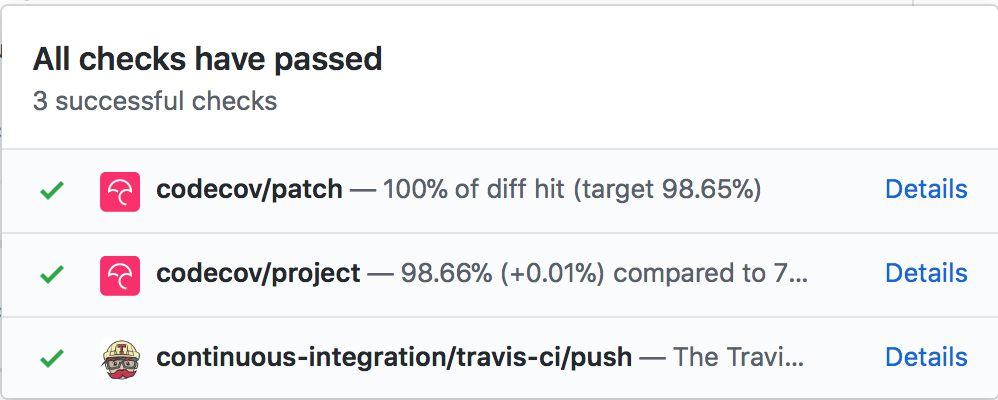
\includegraphics[width=(\linewidth / 3 * 2)]{Chapters/3-RequirementAndSpecifications/github_checks.png}
    \caption{GitHub PR checks}
    \label{fig:github_pr}
\end{figure}

\subsection{Platform requirements}

The application (including the library) has only two dependencies:
\begin{itemize}
  \item A MySQL server
  \item The ability to run Ruby (and Ruby on Rails)
\end{itemize}

\subsection{Specifications for the web application}

\begin{tabularx}{\textwidth}{|c|Y|Y|}
  \hline
  \textbf{R no.} & \textbf{Requirement details} & \textbf{Specification} \\\hline
  \endhead
  R-1 & The web application should be able to store data in a database & Use Ruby on Rails' ActiveRecord to store and access data in a MySQL server \\\hline
  R-2 & The web application should allow users to log-in and keep their data across sessions. & Use devise library for authentication and provide sign-in and sign-up functionality using devise\\\hline
  R-3 &  The web application should allow users to have different roles within the application (e.g.Student/ Teacher/ TA) & Use pundit library for user roles management and authorization\\\hline
  R-4 &  A teacher should be able to create assignments by giving a title, a description, and a SQL query that creates the tables and the relations between them, a SQL query that seeds the table with initial data, and a SQL query which represents the correct answer for the assignment. & Provide a web form built where teachers can create new assignments. The form will be built using Bootstrap, and the code editors should use codemirror to provide code syntax highlighting. \\\hline
  R-5 &  The application should compile the queries provided and if no errors are shown, it will save the assignment in the database and display the schema of the database and the data from it. & Use the compile method provide by the library and defined and display any error that may occur, otherwise save the record in the database. \\\hline
  R-6 & The teacher should allow editing the assignments after they are created. & Recompile the query and update the assignment in the database if no errors are encountered. \\\hline
  R-7 & The teacher should allow the deletion assignments after they are created. & Deletes the challenge from database \\\hline
  R-8 & A student should be able to provide solutions to assignments by submitting a SQL query. The web application should return the results instantly to the students after it assess the query. If any compilation errors are returned, they will be shown to the student. & Provide a web form built in Bootstrap that provides a code editor using codemirror. Assess the query using the assess method provided by grading library. Save all submissions in the database after they have been assessed. \\\hline
  R-9 & A student should be able to view the schema of the database for the assignment. & Render a HTML views that contains the schema of the database and provide a form written in Bootstrap and codemirror where they provide solutions. \\\hline
  R-10 & A  student  should  be  able  to  see  hints  if  they  make  any  errors,  or  they  can  also  see  a breakdown of the components from the teacher’s query and the ones used by their query. & Display a HTML view based on the results of their submission, after being graded. \\\hline
  R-11 & SQL typing on the web application should be made in a browser based code editor that provides syntax highlighting. & Provide a code editor written in codemirror. \\\hline
  R-12 & Teachers should be able to have a graphical view of the results and download the results in  a CSV format.   In  addition,  they  should  be  able  to  view  the  results  of  individual submissions. & Provide a download CSV button that gets the best submission of each student for a certain assignment. Provide a HTML view that displays the result of a individual submission. \\\hline
\end{tabularx}

\subsection{Specification for Library}

\begin{tabularx}{\textwidth}{|c|Y|Y|}
  \hline
  \textbf{R no.} & \textbf{Requirement details} & \textbf{Specification} \\\hline
  \endhead
G-1 & The library should be able to connect to a MySQL server and execute queries on a given database. & Connect to a MySQL database using Ruby library mysql2 \\\hline
G-2 & The library should handle any error that might occur when communicating to the database (including failed execution of SQL queries, connection issues, etc.) and not throw an un-handled error. & Handle errors returned by mysql2 and return library specific errors. \\\hline
G-3 & The library should provide a safe way to execute arbitrary queries that prevents any possible malicious actions (including SQL injection). & Execute the queries in a separate database using a user that has restricted permissions. \\\hline
G-4 & The library should implement a grading algorithm for assessing SQL assignments. & Implement a grading algorithm that follows the grading algorithm defined by XData. That means the grading will compare the components of two canonicalized queries. Therefore, the algorithm will contain two components: the canonicalization of a SQL query and the comparison of components. \\\hline
G-5 & The algorithm should provide a detailed explanation of the grade and how it was assessed. & Return a grade for each component and the components after they have been canonicalized. \\\hline
G-6 & The algorithm should provide hints about how a student could fix his query if the query is wrong & Return the most relevant hint for the query. The relevance of the hint will be determined by two factors: the grade of the component, and a predefined importance ordering of components\\\hline
G-7 & The library should expose a method that allows the compilation of an assignment given a schema query, a seed query and a correct query. The application should return the schema and the data of the database if no errors are encountered. If errors are encountered, then it should return the appropriate error. & Execute the queries and handle any errors if they occur and return them as mentioned in specifications for G-1 and G-2. Extract the tables created in the schema query and then extract the data inserted in the seed query. \\\hline
G- & The library should expose a method that allows the assessment of a submissions given a schema query, a seed query, the instructor's correct query and the submissions' query.  The assessment should be done with the grading algorithm implemented for requirement \ref{req:grading}. The result of the method should be the grade, the explanation implemented for \ref{req:grading_explanation} and the hint returned from the implementation of \ref{req:grading_hint}. & Execute the queries and handle any errors if they occur and return them as mentioned in specifications for G-1 and G-2. Apply the grading algorithm implemented for G-4 and return the grade, the detailed breakdown of the grade implemented for G-5 and the hint from G-6. \\\hline
\end{tabularx}

\chapter{Design}

\section{System Architecture}

As mentioned in section \ref{ch:reqandspec:sec:spec}, we have opted for a design that involves two applications. The main Rails on Rails app includes the grading library as one of its dependencies. In ruby, adding a library as a dependency simply is the equivalent of adding the code of the library directly. That means that the main application can now call the library's code without any other requirement such as running the library independently.

\begin{figure}[h]
    \centering
    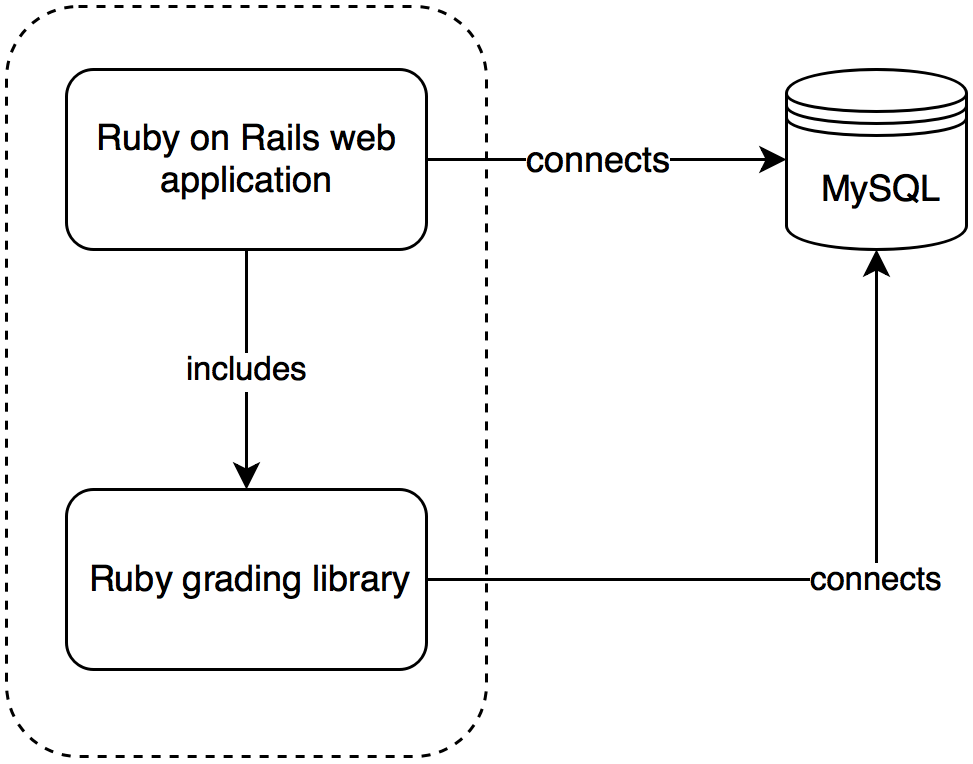
\includegraphics[width=(\linewidth / 2)]{Chapters/4-Design/sysarh.png}
    \caption{System architecture}
\end{figure}

Both the web application and will share the same MySQL server. However, they will both use different databases. A more in-depth explanation of how the library uses the database will be presented in section \ref{ch:impllib:sec:connecting}.

\section{Grading library}

The grading library is composed of multiple modular classes that have a single responsibility. The main entry point of the library is the \mintinline{ruby}{Assessor} class which is the public interface of the library. The library exposes two methods that are called by the main web application:

\begin{itemize}
    \item \mintinline[breaklines]{ruby}{def compile(create_schema_sql_query:, instructor_sql_query:, seed_sql_query:)} which is called by the web application when an exercise is returned. The method checks if the \texttt{SQL} queries submitted by the teacher are correct and if yes, what's the structure of the database.
    \item \mintinline[breaklines]{ruby}{def assess(create_schema_sql_query:, instructor_sql_query:, seed_sql_query:, student_sql_query:)} which returns the results of comparing a student's query with the instructor's query.
\end{itemize}

The library does not have any permanent state so it does not store any compilation results, or submission grades. Therefore, the results returned by these two methods must be saved by the caller if they want them to be stored permanently.

\subsection{Code structure}

As mentioned, one of the goals of the project is to build an application that can be easily extended in the feature. To do this, the library is split in many classes that each handle a very specific feature.

\begin{enumerate}
    \item The \mintinline{ruby}{Assessor} which exposes the public interface of the library.
    \item \mintinline{ruby}{DatabaseConnection} which handles connecting to a database and running single statement queries (queries formed of a single command) and multi statement queries (queries formed of multiple commands). In addition, this class makes sure that data leaks are prevented.
    \item \mintinline{ruby}{DataExtractor} class looks over the extraction of data and schema of a database. This is uses in the \mintinline[breaklines]{ruby}{compile()} method for returning the structure of the database.
    \item \mintinline{ruby}{QueryTransformer} class that handles the canonicalization process. This class sequentially (in a predefined order) runs transformers defined in the \mintinline{ruby}{Trasnformers::} namespace. Each class from the \mintinline{ruby}{Trasnformers::} namespace performs a single type of transformation. They take in a query, apply a set of transformations and then return the transformed query.
    \item \mintinline{ruby}{QueryAttributeExtractor} class which handles the extraction of various components of a query after a transformation has been made. In order to do that, it makes use of parsers defined in defined in the \mintinline{ruby}{Parsers::} namespace. Each class from the \mintinline{ruby}{Parsers::} namespace extracts a single attribute. Although we are using a parser to parse SQL, these classes allow us to remove unwanted syntax and to transformed the parsed elements to a format that suits us better.
    \item \mintinline{ruby}{QueryComparator} class which compares the results of two queries.
    \item \mintinline{ruby}{Graders::} namespace contains multiple graders whose job is to compare a single component of a query (e.g. \mintinline{ruby}{Graders::Columns} handles the assessment of the columns component)
    \item \mintinline{ruby}{QueryComparisonResult} class which represents the final result of the submission. It includes a grade, hint and grades of each component of the query. This class also calculated the partial grade based on the results of the QueryComparator, and a comparison between the actual components of the two SQL queries using the graders from \mintinline{ruby}{Graders::}
    \item In addition, the library also contains multiple \mintinline{ruby}{Error} classes that represent various errors that might happen during the execution of the process - such as the inability to establish a database connection (\mintinline{ruby}{DatabaseConnectionError})
\end{enumerate}

Splitting the functionality into multiple classes leads to cleaner code that allows faster development. This method of development makes use of the Object Oriented Programming principle called encapsulation. Encapsulation, also known as "information hiding", minimizes interdependence between clasess by providing a strong external interface \citep{Encapsulation}. For instance, no class other than \mintinline{ruby}{DatabaseConnection} knows how queries are exactly performed. The other classes simply know that \mintinline{ruby}{DatabaseConnection} provides a way to execute single and multi queries. This allowed the project to initially focus on the core aspect of it - the canonicalization process, before thinking about concurrency or security issues described in section \ref{ch:impllib:sec:connecting}.

\subsection{Compile method}
\begin{figure}[H]
\resizebox{\linewidth}{!}{
    \smartdiagramset{
        uniform sequence color=true,
        sequence item border color=black,
        sequence item text color=white,
        sequence item height=1.5cm
    }
    \smartdiagram[sequence diagram]{
        Create tables,
        Seed initial data,
        Execute correct query,
        Extract tables and data
    }
}
\caption{Overview of compile method}
\end{figure}

When compiling an assessment, a query will go through multiple steps:
\begin{tabularx}{\textwidth}{|c|Y|Y|}
    \hline
    \textbf{Step} & \textbf{Action} & \textbf{Code implementation} \\\hline
    \endhead
    1 & Acquire a database connection and handle any errors & Create a new \texttt{DatabaseConnection} and immediately return any potential \texttt{DatabaseConnectionError}. \\\hline
    2 & Create the database tables passed in the \texttt{create\_schema\_sql\_query} & Execute the \texttt{create\_schema\_sql\_query} on the \texttt{DatabaseConnection} and immediately return any potential \texttt{DatabaseSchemaError} \\\hline
    3 & Seed the database tables data provided by \texttt{seed\_sql\_query} & Execute the \texttt{seed\_sql\_query} on the \texttt{DatabaseConnection} and immediately return any potential \texttt{DatabaseSeedError} \\\hline
    4 & Try to execute the correct query to ensure that the instructor's query can actually be performed
    on the current database and that it does not contain any syntactic errors. & Execute the \texttt{instructor\_sql\_query} on the \texttt{DatabaseConnection} and immediately return any potential \texttt{DatabaseQueryExecutionFailed} \\\hline
    5 & Extract the tables and data from the database & Use \texttt{DataExtractor} to extract data and tables using the \texttt{DatabaseConnection}. \\\hline
\end{tabularx}

\subsection{Assess method}
\begin{figure}[h]
\resizebox{\linewidth}{!}{
    \smartdiagramset{
        uniform sequence color=true,
        sequence item border color=black,
        sequence item text color=white,
        sequence item height=2cm
    }
    \smartdiagram[sequence diagram]{
        Create initial tables and seed data,
        Execute the two queries,
        Canonicalize the queries,
        Extract the components of each query,
        Assign a grade based on components
    }
}
\caption{Overview of compile method}
\end{figure}

The assess method is fairly similar to the compile method. In fact, the steps 1-3 from compile method are also used in this method. The rest of the method continues as following:

\begin{tabularx}{\textwidth}{|c|Y|Y|}
    \hline
    \textbf{Step} & \textbf{Action} & \textbf{Code implementation} \\\hline
    \endhead
    4 & Execute and store the results of both the student's query and the instructor's query & Execute the \texttt{instructor\_sql\_query} and \texttt{student\_sql\_query} on the \texttt{DatabaseConnection} and return any potential \texttt{DatabaseQueryExecutionFailed} \\\hline
    5 & Compare the results obtained in step 4 & Execute \texttt{QueryComparator}'s compare method on the results of the two queries obtained in step 4. \\\hline
    6 & Canonicalize each query & Execute \texttt{QueryTransformer}'s transform method on each query. Internally, each query goes through multiple transformations performed by classes from \texttt{Transformers::} namespace. \\\hline
    7 & Extract the components of each query &  Execute \texttt{QueryAttributeExtractor}'s extract method on each query. Internally, each query component is obtained by multiple parsers performed by classes from \texttt{Parsers::} namespace. \\\hline
    8 & Compute the final grade and return the components, hints and grade to the caller &  Build a new \texttt{QueryComparisonResult}'s based on the result of the comparison of the results, and the components obtained in step 6. Internally, the partial grade is obtained by comparing each element. The comparison of each component is delegated to a class from \texttt{Graders::} namespace. Finally, assemble the final \texttt{QueryComparisonResult} which includes the full list of components, a hint based on the comparison, and the final grade\\\hline
\end{tabularx}


\begin{tabularx}{\textwidth}{|c|Y|Y|}

\end{tabularx}

\section{Web application}


As described in the requirements section (\ref{ch:reqandspec:sec:rec}) for the web application, the main purpose of the web application is to provide a CRUD (create, read, update and delete) web interface. Ruby on Rails provides a fairly standardized way of creating applications, with little margin for different designs, as the framework is very opinionated using what is commonly known as \textit{convention over configuration} \citep{ruby_on_rails}.

Ruby on Rails uses a Model-View-Controller (MVC) as an architectural pattern. Ruby on Rails provide three main sub-frameworks to handle each component of the MVC pattern \citep{ruby_on_rails}:
\begin{itemize}
    \item \textbf{M}: \mintinline{ruby}{ActiveRecord} which handles the connection between the \textit{domain objects} and the database
    \item \textbf{V}: \mintinline{ruby}{ActiveView} which presents data in various formats including \texttt{HTML}, \texttt{CSV}, etc.
    \item \textbf{C}: \mintinline{ruby}{ActionController} which receives web requests and returns views to users.
\end{itemize}
As \texttt{RoR} uses MVC we can easily identify each component of the web application based on this pattern.

\subsection{Models}

Models represents the domain of the project \citep{ruby_on_rails} or the state of the application \citep{ruby_on_rails_book}. While the state can also be transient, most models are permanent and to preserve them we will store them in the database. \mintinline{ruby}{ActiveRecord} provides a object relation mapping (ORM) from \texttt{Ruby} objects to \texttt{SQL}. The domain of the application contains the following models:
\begin{itemize}
    \item \mintinline{ruby}{User} which represents a user of the web application. A user has an email and a role (either student or teacher). In addition every user has a password that they use to authenticate on the website.
    \item \mintinline{ruby}{Challenge} which represents an assignment created by a teacher. A challenge has a title, content, and three \texttt{SQL} queries: the query for creating the database schema, the query for seeding the initial data, and the correct solution for the assignment.
    \item \mintinline{ruby}{Submission} which represents a submission created by a student to a challenge based on a student's query. A submission stores two important attributes: meta-data which contains a breakdown of each component of the query after canonicalization, a final grade, and a grade for each component. Finally, a submission might store a hint if the query is wrong.
\end{itemize}

The application also defines the following relations between models:
\begin{itemize}
    \item A \mintinline{ruby}{Challenge} belongs to an author (an \mintinline{ruby}{User})
    \item A \mintinline{ruby}{Submission} belongs to an author (an \mintinline{ruby}{User}) and to \mintinline{ruby}{Challenge}.
    \item A \mintinline{ruby}{Challenge} has many \mintinline{ruby}{Submission}s
    \item A \mintinline{ruby}{User} has many \mintinline{ruby}{Submission}s
\end{itemize}

As the models are also represented in the database, each model will also be represented by a table in the database. The database has the following enhanced entity-relationship (EER) diagram:

\begin{figure}[h]
    \centering
    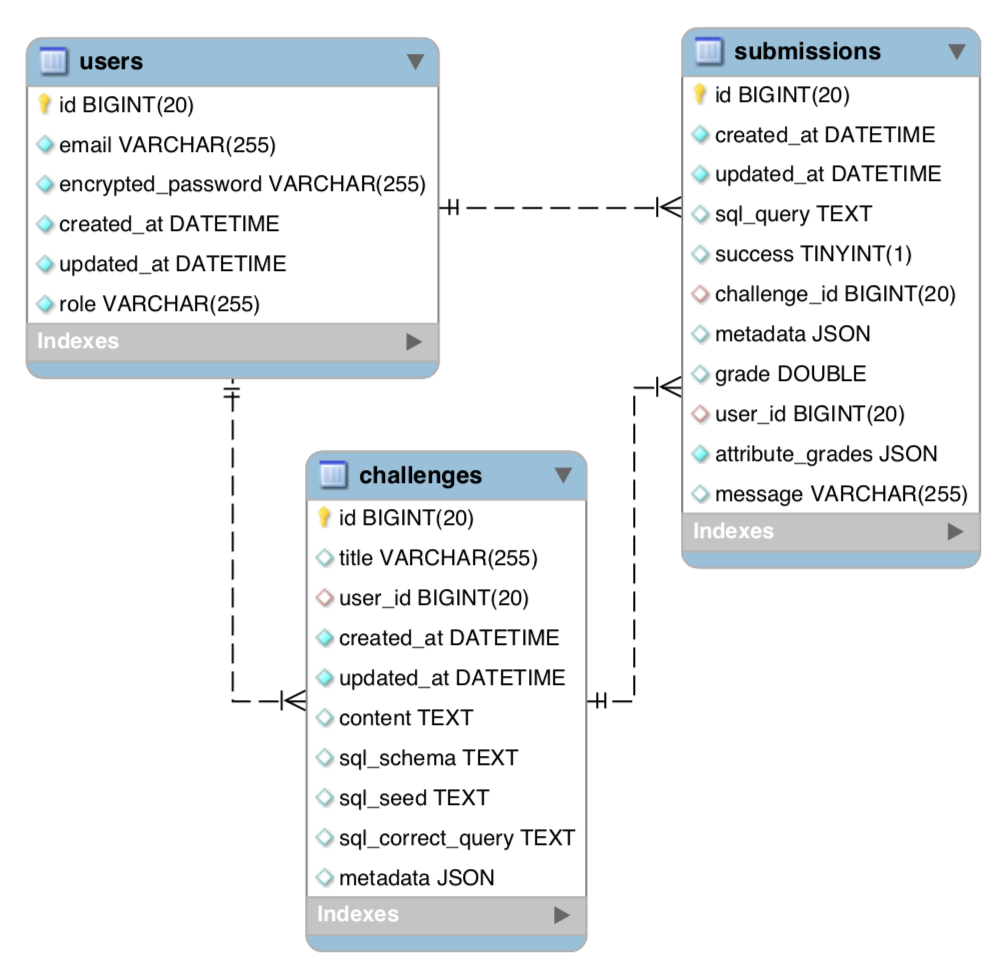
\includegraphics[width=\textwidth/3*2]{Chapters/4-Design/database_schema.png}
    \caption{EER diagram of the web application}
\end{figure}

\subsection{Views}

The role of views in a \texttt{MVC} application is to render data \citep{ruby_on_rails}. Most of the application is rendered in \texttt{HTML} (using \mintinline{ruby}{ActionView}) which is displayed in user's browser. The application includes multiple views that serve different purposes: displaying forms, displaying challenge details, etc.

\subsection{Controllers}

The role of controllers is to \textit{orchestrate} the application. They receive user input (in the form of HTTP requests in the case of Ruby on Rails applications) and returns the correct views which display the correct models \citep{ruby_on_rails_book}. Controllers are implemented as subclasses of \mintinline{ruby}{ActionController::Base} in \texttt{RoR}. This super-class already knows how to handle HTTP requests and return the response to the user. In general, controllers in Ruby on Rails implement the Representational State Transfer (REST) actions. RESTful web services make use of the HTTP methods as following \citep{rodriguez2008restful}:

\begin{tabularx}{\textwidth}{|c|X|X|X|}
    \hline
    & \textbf{URL} & \textbf{Ruby on Rails action name} & \textbf{Result} \\\hline
    GET & /resource\_name & index & Get all resources \\\hline
    GET & /resource\_name/:id & show & Get resource with given id \\\hline
    GET & /resource\_name/new & new & Get the form for creating a new resource \\\hline
    GET & /resource\_name/:id/edit & edit & Get the form for editing a resource with given id \\\hline
    POST & /resource\_name & create & Create resource \\\hline
    PUT & /resource\_name/:id/ & update & Update a resource with a given id \\\hline
    DELETE & /resource\_name/:id & destroy & Get resource with given id \\\hline
\end{tabularx}

REST Ruby on Rails controllers have in general, in general, the following structure \citep{RoRDocumentation}:
\begin{enumerate}
    \item Receive a web request
    \item Fetch and optionally modify a model
    \item Return a view to the user
\end{enumerate}

The web application built in this project includes the following controllers:
\begin{enumerate}
    \item \textbf{Authentication and user-related controllers}: these controllers handle the basic user management tasks. They are provided by a 3rd-party library called \texttt{devise}.
    \item \mintinline{ruby}{ChallengesController} which defines the REST actions for managing \mintinline{ruby}{Challenge}
    \item \mintinline{ruby}{SubmissionsController} which defines the REST actions for managing \mintinline{ruby}{Submissions}

\end{enumerate}

\section{Example of interaction between user, web application and library and database}

\begin{figure}[h]
    \centering
    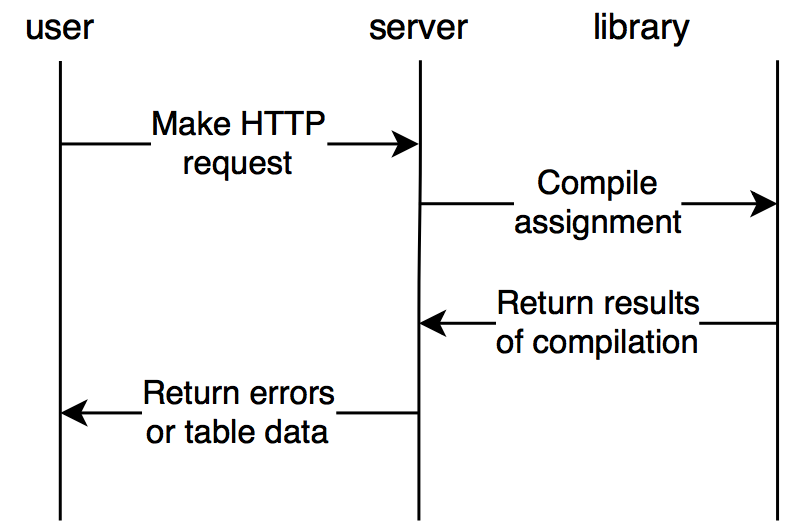
\includegraphics[width=(\linewidth / 2)]{Chapters/4-Design/create_assignment.png}
    \caption{Overview of creating a new assignment}
    \label{fig:create_assignment}
\end{figure}

The user never interacts directly with the library or the database system as all communication from user's perspective is done from the web application.

An example of such an interaction can be seen in figure \ref{fig:create_assignment}. The user makes a POST HTTP requests which is handles by the the Ruby on Rails web application in the \mintinline{ruby}{create} action from \mintinline{ruby}{ChallengesController}. Internally, the controller checks authentication and makes sure the user has the permission to create an assignment. After these checks are made, it then passes on SQL queries received to the library. The library compiles these queries and returns the results or errors. If there are no errors, the tool will create a new \mintinline{ruby}{Challenge} and return a success message to the user as a rendered HTML view. If errors are encountered, they are also rendered to the user as HTML, but no challenge is saved as the submitted parameters were not be valid.

A similar interaction also occurs when a student submits a solution to an assignment created by an instructor. However,

\chapter{Implementation and testing}

\section{Library: connecting to a MySQL server and executing queries} \label{ch:impllib:sec:connecting}
To connect to a MySQL server, the application uses the Ruby library mysql2. The library, or gem as it's called in Ruby, provides the implementation for connecting, querying and retrieving results from a MySQL server. mysql2 is a binding to MySQL's C library libmysql. mysql2 is the more modern and lean version of the mysql version. Compared to mysql gem, mysql2 gem can be 2 times faster and is built with Ruby in mind. Furthermore, mysql2 is also much more popular with over 42 million downloads on RubyGems, compared to mysql's 8 million downloads.

To connect to a MySQL server, the library requires the address and port of the server, and an account and password. The account must be the root user or at least one that has the permission to create and drop databases, to create and drop users, and to grant permissions to an user.

\subsection{Handling concurrent submissions}

As the library will be used in a web application, concurrency is inevitable. Users can submit solutions at any time and it is possible that two users submit solutions at the same time. Obviously, concurrency can be ignored by limiting the execution of only one compile or assessment at a time. However, this solution can lead to frustrating waiting times and requires the implementation of background workers to compile the work. Therefore, the tool opted to implement a solution that allows concurrent executions.

To allow concurrency, each submission or compilation is performed using different connections to different databases (a MySQL server can have multiple databases).  Every compilation or submission begins by creating a new and unique database based on the current time. The database name will follow the format \texttt{HOURMINUTESECOND}. While this should cover most cases, due to the concurrent nature of the application, it might be the case that two connections try to create a database with the same name. However, MySQL statements are atomic. That means that two statements can not both change the schema of the MySQL server. Therefore, it is guaranteed that at least one create will fail. In this case, we repeat all failed creations (by using the new time) until they succeed. On second and further attempts, we also add a \mintinline{ruby}{_attempt} at the end of the database name to reduce the chance of another conflict. At the end of the compilation, the newly created database will be dropped and all data associated discarded.

%TC:ignore
\begin{code}
    \begin{minted}{ruby}
success = false
attempt = 0
while !success do
  time = DateTime.now

  if attempt > 0
    @database = "#{Time.now.strftime("%H%M%S")}_#{attempt}"
  else
    @database = "#{Time.now.strftime("%H%M%S")}"
  end

  begin
    @client.query("CREATE DATABASE `#{@database}`")
    success = true
  rescue Mysql2::Error => exception
    raise exception unless exception.message.include?("database exists")
    success = false
    attempt += 1
  end
end
\end{minted}
    \caption{Creating a new database for each run}
    \label{fig:creating_new_database}
\end{code}
%TC:endignore

\subsection{Preventing malicious actions from input SQL queries}

Considering the fact that the library executes arbitrary queries, the risks associated with malicious SQL are significant. The application never returns back the query results which means that the potential for data leaking through this does not exist. However, an arbitrary query can destroy or modify other databases on the MySQL server. Therefore, the library must take extra precautions as it deals with unchecked user code. To prevent malicious actions, we create a new MySQL user that only has permission for the newly created database.

%TC:ignore
\begin{code}
\begin{minted}{ruby}
@client.query("CREATE USER IF NOT EXISTS `#{@database}`;")
@client.query("GRANT ALL PRIVILEGES ON `#{@database}`.* TO `#{@database}` WITH GRANT OPTION;")
\end{minted}
\caption{Creating a new user with permissions for the new database}
\label{fig:creating_new_user}
\end{code}
%TC:endignore
All used queries are performed using this user, instead of using the root one. The temporary user is also deleted at the end of the compile/ assessment execution. This way, the user input can only damage the created database for his assessment. However, this is not an issue considering these are short-lived databases which are destroyed at the end of the assessment.

The only way to get around the limitation of the restricted user would be to use a different user. Changing the user in MySQL is not possible through a MySQL command. The only possible way would be to use the \texttt{system} command which executes bash code in combination with the \texttt{mysql -uroot --password} bash command if they knew the root password, but not the url of the database. However, the \texttt{system} command is only available on connections opened with the \texttt{mysql} bash command, which is not the case for \texttt{mysql2} - so users can not exploit this method. Furthermore, the user has limited permissions so he can not run commands such as \mintinline{mysql}{SET PASSWORD} to change existing users.

\section{Library: parsing and transforming queries}

Part of the canonicalization and grading process, SQL queries will go through multiple transformations after being parsed and separated in independent components. MySQL does not provide an official parser for any programming language, so the library had to use a 3rd party tool. The advantage of using an existing parser is that we can ignore the implementation details of parsing.

The library initially used the Ruby gem sql-parser. Throughout the development process, there have been multiple problems associated with this tool. Most importantly, the library did not have support for multiple SQL statements that we required. Unfortunately, many issues with sql-parser were discovered only late in the project.

An alternative was represented by pg\_query Ruby gem. Internally it uses PostgreSQL's parsing library libpg\_query built in C++. pg\_query provides much better code and stability, due to its nature of being part of a production database system, compared to sql-parser which was only used for parsing. PostgreSQL, like MySQL, is a database system that is widely used, being the 4th most used database engine according to \cite{db_engine:statistics}. Although both PostgreSQL and MySQL have SQL at their core, each one implements their own version of SQL. Therefore, a query might work in MySQL, but not work in PostgreSQL, or return different results. For instance, in MySQL string comparison is case insensitive, while PostgreSQL is not. In addition, each SQL version adds their own functions that diverge from Standard SQL. Therefore, implementing pg\_query turned out to be impossible due to the many differences in syntax between them. In addition, time constraints made it unjustifiable to spend time on re-implementing all transformers already built.

\subsection{Extending sql-parser}

In the end, due to the issues described previously, a decision was made to continue using sql-parser. Fortunately, sql-parser uses a MIT license which allowed us to fork the library and implement the fixes in the fork. The parser was implemented using Racc's grammar files. According to the GitHub page of the tool, Racc is a \textit{LALR(1) parser generator} that generates Ruby code. LALR parsers are also known as "Look Ahead Left to Right" parsers. The fork created implemented the following functionality:
\begin{itemize}
    \item Support for \mintinline{mysql}{DISTINCT}, \mintinline{mysql}{DISTINCTROW}, \mintinline{mysql}{ALL} in \mintinline{mysql}{SELECT} statements
    \item Support for \mintinline{mysql}{LIMIT} and \mintinline{mysql}{OFFSET}
    \item Support for using a qualified column in \mintinline{mysql}{ORDER BY} clause
    \item Support for using the columns number in \mintinline{mysql}{GROUP} clause
    \item Support for using subqueries in \mintinline{mysql}{FROM} clause
\end{itemize}

The process of adding a new feature was formed of multiple parts:
\begin{enumerate}
    \item Create a \mintinline{ruby}{Node} class representing the new clause, if a new clause was implemented. A \mintinline{ruby}{Node} represents an element of a query: a clause, a number, a word, a condition, etc. For instance, the newly created \texttt{LIMIT} node has the following structure:
    \begin{code}\centering
\begin{minted}{ruby}
class LimitClause < Node
    def initialize(limit, offset)
        @limit = limit
        @offset = offset
    end

    attr_reader :limit, :offset
end
\end{minted}
\caption{Limit clause \mintinline{ruby}{Node}}
\label{fig:limit_clause}
\end{code}
    \item Update existing \mintinline{ruby}{Node} to link to the newly created node. For instance, the \mintinline{ruby}{LimitClause} node had to be linked to the \mintinline{ruby}{TableExpression} node.
    \item Add the new parsing rules to Racc grammar file. For instance, when adding the LIMIT clause there are three options: there is only a limit number, there are two numbers for limit and offset separated by the word \texttt{OFFSET}, or the two numbers are separated by a comma:
\begin{code}
    \centering
    \begin{minted}{ruby}
  limit_clause
: # no action
| LIMIT unsigned_integer { result = SQLParser::Statement::LimitClause.new(val[1], nil) }
| LIMIT unsigned_integer OFFSET unsigned_integer { result = SQLParser::Statement::LimitClause.new(val[1], val[3]) }
| LIMIT unsigned_integer comma unsigned_integer { result = SQLParser::Statement::LimitClause.new(val[3], val[1]) }
    \end{minted}
    \caption{Limit clause \texttt{Racc}}
    \label{fig:limit_clause_racc}
\end{code}
\end{enumerate}

\subsection{Using sql-parser to parse SQL queries}
Using sql-parser to parse SQL queries is straight forward. The library provides the \mintinline{mysql}{scan_str} which transform a string (the SQL query) into a SQL Abstract Syntax Tree (AST). The AST is formed of multiple nodes. As previously mentioned in the lat section, a node is a component of the clause. The general structure of the AST for a SELECT query has the following structure is represented in figure \ref{fig:select_ast}.

\begin{figure}[ht]
\centering
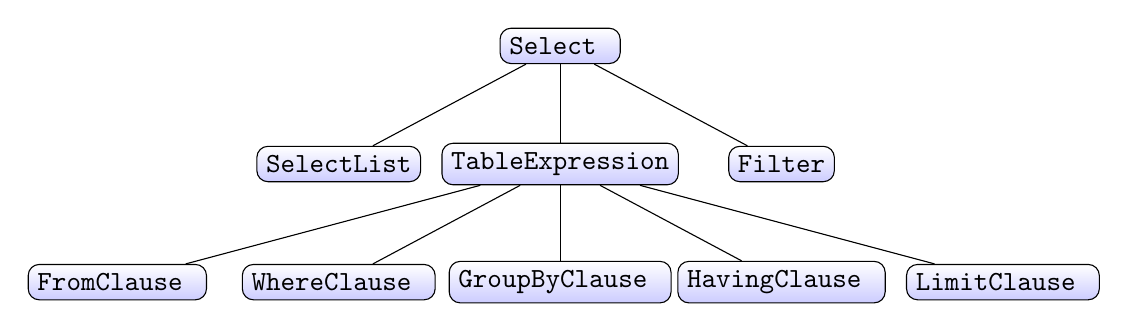
\begin{tikzpicture}[sibling distance=8em,
  every node/.style = {shape=rectangle, rounded corners,
    draw, align=center,
    top color=white, bottom color=blue!20}]]
  \node { \ttfamily Select }
    child { node {\ttfamily SelectList} }
    child { node {\ttfamily TableExpression}
        child { node {\ttfamily FromClause } }
        child { node {\ttfamily WhereClause } }
        child { node {\ttfamily GroupByClause } }
        child { node {\ttfamily HavingClause } }
        child { node {\ttfamily LimitClause } } }
    child { node {\ttfamily Filter} };
\end{tikzpicture}
\caption{General structure of the SELECT's AST}
\label{fig:select_ast}
\end{figure}
All the leaves presented in figure \ref{fig:select_ast} also have their nodes. For instance, SelectList has an array of columns which can be of many types (QualifiedColumn, Column, AggregateColumn). In addition, what we previously called Boolean components (WHERE and HAVING) have both subtrees representing the Boolean expression.


\subsection{Using sql-parser to change queries}
sql-parser also provides a way to change a parsed query (which is now a combination of multiple Nodes) back to a SQL query. Unfortunately, the process of internally modifying the structure of a query is not well-defined and there is no public interface exposed. Each node has one or more private instance variable that represent the values of the Node. For instance, the limit node shown in listing \ref{fig:limit_clause}, has two such variables: limit and offset. sql-parser does not provide a way to change these properties as all Nodes just expose a reader method (set using \mintinline{ruby}{attr_reader}). Fortunately, ruby provides a \mintinline{ruby}{instance_variable_set} method while allows anyone with a reference to an object to change that object's internal variables even if they are private and no setter is exposed. It is worth mentioning that while this approach might work, the use of this method \mintinline{ruby}{instance_variable_set} goes against the principle of encapsulation, and might mean that a future update to the library can lead to errors, if the internal structure of Nodes is modified.

\begin{code}
\begin{minted}{ruby}
@parsed_query.query_expression.list.instance_variable_set(
  "@columns",
  new_columns
)
\end{minted}
\caption{Example of updating the column list for a parsed query}
\end{code}

After a query is modified, sql-parser exposes a \mintinline{ruby}{.to_sql} method on each Node that can be used to transform a Node to a SQL statement.

\section{Library: handling sub-queries}

Unfortunately, compared to XData, the library can not handle submissions with XData. Some work to implement this has been attempted and is available in the current code: canonicalization of sub-queries, comparison of nested queries, updating sql-parser to support sub-queries in the FROM clause, etc. Unfortunately, this work has been added very late in the project which meant that most existing work had to be redone. The work had to be redone because some parts of the library made the assumption that no sub-queries are present. For instance, the library contains multiple canonicalizations that make use of nested sub-queries. 

If the library will encounter a sub-query, it will return an error explaining that such SQL queries are not currently supported.

\section{Library: canonicalizing queries}

As previously mentioned in section \ref{ch:lit:sec:improved_canon}, the library will implement a canonicalization step. The library implements all canonicalizations done by XData and described in section \ref{ch:lit:sec:canonicalization}, and the additional ones presented in section \ref{ch:lit:sec:improved_canon}. All transformations use sql-parser's transformations ability combined with the ability to make queries on the database.

As mentioned in the design section \ref{ch:lit:sec:improved_canon}, the canonicalization process is done sequentially in a specific order that ensures that later canonicalizations do not make changes that make changes incompatible with previously executed transformations. 

\begin{code}
\begin{minted}{ruby}
def transform(query)
  TRANSFORMERS.each do |transformer_class|
    query = transformer_class.new(@connection).transform(query)
  end

  query
end
\end{minted}
\caption{Sequential transformation of a query}
\label{fig:sequential transformation of a query}
\end{code}

\subsection{Transforming \mintinline{mysql}{*} to all columns}
To transform \mintinline{mysql}{*} to MySQL, the library uses the fact that it doesn't need to support sub-queries. That means that it can simply look at what tables are selected and then perform \mintinline{mysql}{SHOW COLUMNS FROM table_name} on each table to get the full list of columns for each table. The library will then simply update the list of columns (initially represented by a \mintinline{mysql}{*}) to the new list of columns which contain the full list of \texttt{table\_name.column} for each selected table.

\begin{code}
\begin{minted}{ruby}
new_columns = table_list.map do |table|
  columns_query = "SHOW COLUMNS from #{table}"
  columns = @connection.query(columns_query).map { |k| k["Field"] }

  columns.map do |column_name|
    SQLParser::Statement::QualifiedColumn.new(
      SQLParser::Statement::Table.new(table),
      SQLParser::Statement::Column.new(column_name)
    )
  end
end.flatten
\end{minted}
\caption{Getting the full list of columns for a query}
\end{code}

\subsection{Transforming ambigous columns to unambigous columns}
Transforming ambiguous columns to unambiguous columns is done in a similar way as the previous transformations. The transformation makes use of two important aspects:
\begin{enumerate}
    \item One can determine the full list of columns for each table expression component, by running \mintinline{mysql}{SHOW COLUMNS FROM table_name}.
    \item An ambiguous column can belong to a single table from a query. If a column cannot be made qualified, then MySQL will automatically return the \textit{column xx in field list is ambiguous''} error.
\end{enumerate}

Therefore to transform an ambiguous column we must go through the full list of columns of each table until we find a match. We then transform the ambiguous column to a qualified column. This process can be seen in listing \ref{fig:find_table}.

An additional type of ambiguous column type is the position reference one which is found in the GROUP and ORDER clauses. In these two clauses, one can write \mintinline{mysql}{ORDER BY 2} where 2 references the second column from the select list. To find the qualified column that the position column references we need to look at the select list (after it was transformed to qualified columns) and select the right position: \mintinline{ruby}{@parsed_query.query_expression.list.columns[column.value - 1]} (position columns start at index 1, while arrays start at 0 in ruby).

Finally, the library also considers the aggregate column types which inside might contain a ambiguous column as well. Aggregate columns are of type \mintinline{ruby}{SQLParser::Statement::Aggregate} which has an attribute of type column. Therefore, we need to apply the same transformation to the inner column attribute.

In sql-parser, unqualified columns have the parsed node type \mintinline{ruby}{SQLParser::Statement::Column}, while qualified columns have the parsed node type \mintinline{ruby}{SQLParser::Statement::QualifiedColumn}.

%TC:ignore
\begin{code}
\begin{minted}{ruby}
def find_table_for(column_name)
  table_list.detect do |table|
    columns_query = "SHOW COLUMNS from #{table}"
    columns = @connection.query(columns_query).map { |k| k["Field"] }
    columns.include?(column_name)
  end
end
\end{minted}
\caption{Determining the table for an ambigous column with name}
\label{fig:find_table}
\end{code}
%TC:endignore


\subsection{Transforming equivalent columns}

The transformation of equivalent columns is a two step process. First, the library determines which components are equivalent, and after that it updates all column references to the minimum lexicographically string from the equivalence group.

To determine the equivalent columns the library builds a undirected graph $G(V, E)$:
\begin{enumerate}
    \item $V$: the list of all columns used in the table expression
    \item $E$: there is an edge between $v_1$ and $v_2$ if and only if in the table expression there is a join condition based on the equality of $v_1$ and $v_2$. To build the edges, the library goes over all join conditions from the SQL statement and builds the edges as described above.
\end{enumerate}

We can then apply a strongly connected component (SCC) algorithm to obtain all SCCs from a graph. If a column $v$ belong to component $c$, then it means that $v$ is equivalent to all other $v_e$, where $v_e \in c$.

\begin{figure}[H]
\begin{tabular}{ c c }
\begin{minipage}[t]{0.5\textwidth}
\begin{minted}{mysql}
SELECT *
FROM table1
LEFT JOIN table2 on table1.id = table2.fid
LEFT JOIN table3 on table2.fid = table3.random_id
\end{minted}
\end{minipage}
&
\raisebox{-.5\height}{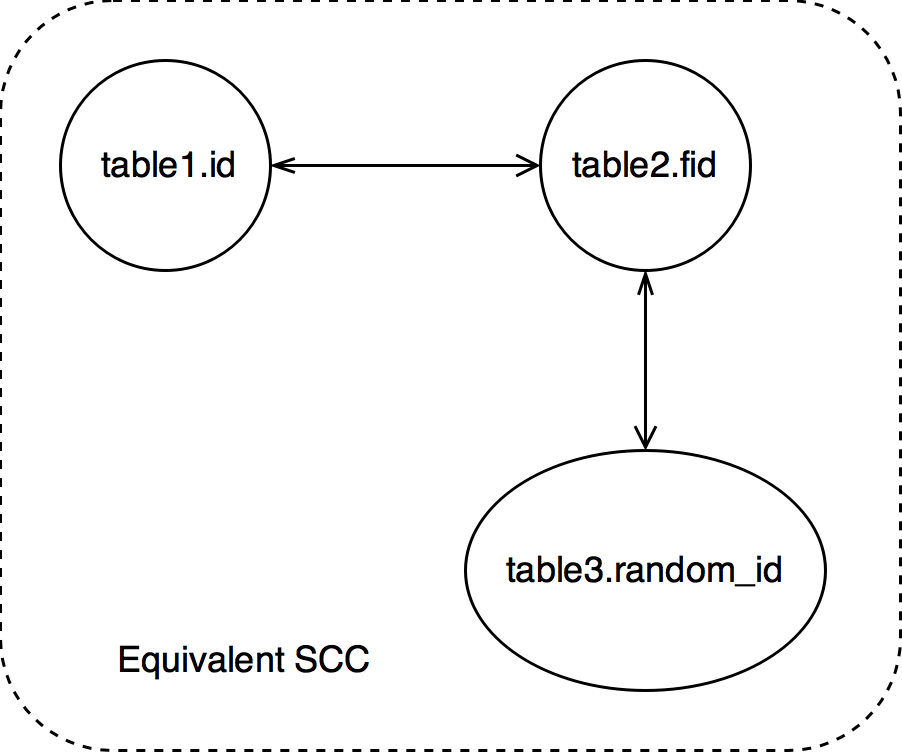
\includegraphics[height=4cm]{Chapters/5-Implementation/scc.png}}
\end{tabular}
\caption{Example of equivalence graph}
\end{figure}

To build the graph we use a Ruby library called RGL. RGL provides the implementation of various graph structures and graph algorithms (including the SCC algorithm).

\begin{code}
\begin{minted}{ruby}
equivalence = equivalences_list.detect do |equivalences|
  equivalences.include?(column.to_sql)
end

if equivalence.present?
  # transform qualified columns in sql form to two strings representing the
  # table and the column name
  table_name, column_name = equivalence.sort.first.remove("`").split(".")

  SQLParser::Statement::QualifiedColumn.new(
    SQLParser::Statement::Table.new(table_name),
    SQLParser::Statement::Column.new(column_name)
  )
else
  column
end
\end{minted}
\caption{Transforming equivalent columns}
\end{code}

\subsection{Transforming conditions from WHERE, HAVING, and JOIN contiions}
The WHERE and HAVING clauses and the JOIN conditions are represented by a Boolean expression tree. When transforming these clauses it is essential to ensure that the structure of the expression is not altered - that is the before and after expressions are equivalent. To do this, the algorithm traverses the tree recursively and only replaces leafs with either another leaf (in the case of transforming a condition to another) or to a inner node that has two leaves (in the case of transforming a condition to multiple another).

\begin{code}
\begin{minted}{ruby}
def transform_between_queries(statement)
  if statement.is_a?(SQLParser::Statement::SearchCondition)
    statement.class.new(
      transform_between_queries(statement.left),
      transform_between_queries(statement.right)
    )
  elsif statement.is_a?(SQLParser::Statement::Between)
    transform_between_query(statement)
  else
    statement
  end
end
\end{minted}
\caption{Example of traversing a Boolean expression tree}
\end{code}

\subsubsection{Transforming \mintinline{mysql}{BETWEEN} predicate}

A \mintinline{mysql}{column BETWEEN a AND B} predicate will be transformed to two separate predicates: \mintinline{mysql}{column >= a} and \mintinline{mysql}{column <= b}. 

\begin{code}
\begin{minted}{ruby}
def transform_between_query(predicate)
  SQLParser::Statement::And.new(
    SQLParser::Statement::GreaterOrEquals.new(predicate.left, predicate.min),
    SQLParser::Statement::LessOrEquals.new(predicate.left, predicate.max)
  )
end
\end{minted}
\caption{Transforming a BETWEEN predicate}
\label{fig:transforming_a_betweeb}
\end{code}

\subsubsection{Transforming \mintinline{mysql}{NOT} comparison predicates}

In the case of \mintinline{mysql}{NOT} predicates, the transformation process simply transforms the predicate to its opposite:
\begin{enumerate}
    \item \mintinline{mysql}{>} becomes \mintinline{mysql}{<=}
    \item \mintinline{mysql}{>=} becomes \mintinline{mysql}{<}
    \item \mintinline{mysql}{<} becomes \mintinline{mysql}{>=}
    \item \mintinline{mysql}{>=} becomes \mintinline{mysql}{>}
\end{enumerate}

In addition to these 4 predicate types, NOT can also be used with other types of predicates which the library will not transform (e.g. \mintinline{mysql}{NOT LIKE} which cannot be easily transformed to remove the use of \mintinline{mysql}{NOT}).

\begin{code}
\begin{minted}{ruby}
def transform_not(not_statement)
  # Greater
  if not_statement.value.is_a?(SQLParser::Statement::Greater)
    SQLParser::Statement::LessOrEquals.new(not_statement.value.left, not_statement.value.right)
  elsif not_statement.value.is_a?(SQLParser::Statement::GreaterOrEquals)
    SQLParser::Statement::Less.new(not_statement.value.left, not_statement.value.right)
  # Less
  elsif not_statement.value.is_a?(SQLParser::Statement::Less)
    SQLParser::Statement::GreaterOrEquals.new(not_statement.value.left, not_statement.value.right)
  elsif not_statement.value.is_a?(SQLParser::Statement::LessOrEquals)
    SQLParser::Statement::Greater.new(not_statement.value.left, not_statement.value.right)
  else
    not_statement
  end
end
\end{minted}
\caption{Transforming NOT}
\label{fig:transforming_not}
\end{code}

\subsubsection{Transform \mintinline{mysql}{>} and \mintinline{mysql}{>=} to \mintinline{mysql}{<} and \mintinline{mysql}{<=}}

Transforming \mintinline{mysql}{>} and \mintinline{mysql}{>=} to \mintinline{mysql}{<} and \mintinline{mysql}{<=} is done by simply reverting the predicate and the switching the left element of the comparison predicate with the right element of the predicate.

\begin{code}
\begin{minted}{ruby}
def transform_comparison_predicate(predicate)
  if predicate.is_a?(SQLParser::Statement::Greater)
    SQLParser::Statement::Less.new(
      predicate.right,
      predicate.left
    )
  elsif predicate.is_a?(SQLParser::Statement::GreaterOrEquals)
    SQLParser::Statement::LessOrEquals.new(
      predicate.right,
      predicate.left
    )
  else
    predicate
  end
end
\end{minted}
\caption{Transforming \mintinline{mysql}{>} and \mintinline{mysql}{>=} to \mintinline{mysql}{<} and \mintinline{mysql}{<=}}
\label{fig:transforming_great}
\end{code}

\section{Library: extracting attributes from a canonicalized query}

While sql-parser provides the AST tree for the parsed query, it does not explicitly provide the components of a query. To extract them, the library makes use of the AST and makes various transformations in order to extract the components to a desired data structure. The resulting data structure might be similar to the AST (which is true for most components), but it might also be different (for instance the FROM expression is represented as a tree in the AST, but we can more clearly represent it as an array).

These extraction and transformation process help in two important ways. First of all, it extracts the data in a format that can be easily compared and identical across similar types of expressions (for instance the structure of the WHERE component is identical to the structure of the HAVING component). In addition, the format can be defined in a way that is also easy to display on the front-end.

\subsection{Making defaults explicit}

Every \texttt{MySQL} query has certain default attributes. For instance, every \texttt{MySQL SELECT} query has a default uniqueness filter of \mintinline{mysql}{ALL}. That means while explicitly mentioning \mintinline{mysql}{ALL} will have no effect, it does not mean that it is making the query wrong. In order to accurately compare two queries, we must make the defaults explicit in both queries. The defaults will be made explicit during this extraction process.

\subsection{Format of components}

\begin{itemize}
    \item \textbf{Selected columns} are simply represented as an array of strings, where every string represents a selected column.
    \item \textbf{Order by} clause is represented represented as an array of strings, where every string represents a column.
    \item \textbf{Group} clause is represented represented as an array of strings, where every string represents a column.
    \item \textbf{Tables} clause is represented represented as an array of hashes. There are two types of hashes that can be included:
    \begin{enumerate}
        \item The first element of the array is the base table (or sub-query) of the \mintinline{mysql}{FROM} clause. The item is represented as a hash containing the following keys:
        \begin{enumerate}
            \item \mintinline{ruby}{type}: either \mintinline{ruby}{"table"} or \mintinline{ruby}{"Subquery"}
            \item \mintinline{ruby}{table}: the table name or \mintinline{ruby}{attributes} in the case of sub-queries
            \item \mintinline{ruby}{sql}: the element represented a SQL expression
        \end{enumerate}
        \item The other elements (the joined tables or joined sub-queries) of the array are represented as a hash containing the following keys:
        \begin{enumerate}
            \item \mintinline{ruby}{join_type}: the type of the join
            \item \mintinline{ruby}{table}: a hash that represents a table or sub-query. The format of the hash is the same one as the first element of the array.
            \item \mintinline{ruby}{searchcondition}: represents the join condition. Even if the search condition is similar to a Boolean component, at the moment, the join condition is represented simply as a string. The implication of this representation is that no partial grading is possible on the search condition.
            \item \mintinline{ruby}{sql}: the full SQL expression for the join (e.g. \mintinline{mysql}{LEFT JOIN table_name ON condition1 AND CONDITION 2})
        \end{enumerate}
    \end{enumerate}
    \item \textbf{Distinct filter} is represented a simple string.
    \item \textbf{Limit} clause is represented as a hash with two keys: limit and offset. If the limit is not defined then the value \texttt{inf} will be associated with it.
    \item \textbf{Where and Having} clauses are represented identically. There are two formats in which the library represents them as each format is used for a different purpose:
    \begin{enumerate}
        \item For the grading algorithm, these clauses are represented as binary trees.
        \item For the web application, these clauses are represented as trees (but not binary trees), where search conditions (e.g. \mintinline{mysql}{AND}) can have more than two children. For instance, the binary tree for expression ($ a \land b \land c$) has the following structure: 
        
\Tree[
    .$\land$
    [
        .$\land$
        [.$a$ ]
        [.$b$ ]
    ]
    [
        .$c$
    ]
]

while the tree format for the web application has the following structure

\Tree[
    .$\land$
    [
        .$a$
    ]
    [
        .$b$
    ]
    [
        .$c$
    ]
]

This format allows easier display on the front-end of the conditions.
    \end{enumerate}
\end{itemize}


\section{Library: partial grading}

\begin{code}
\begin{minted}{ruby}
def match_score(column1, column2)
  if column1 == column2
    2
  else
    table_name1, column_name1 = column1.split('.')
    table_name2, column_name2 = column2.split('.')

    if table_name1 == table_name2
      2.0 / levenshtein_distance(column_name1, column_name2)
    else
      0
    end
  end
end
\end{minted}

\caption{Match score for columns}
\end{code}

\begin{code}
\begin{minted}{ruby}
def grade
  if @student_distinct == @instructor_distinct
    1.0
  elsif @student_distinct == 'DISTINCT' && @instructor_distinct == 'DISTINCTROW'
    0.5
  elsif @student_distinct == 'DISTINCTROW' && @instructor_distinct == 'DISTINCT'
    0.5
  else
    0
  end
end
\end{minted}
\caption{Partial grading of distinct filter}
\end{code}

\section{Library: providing hints}

Currently, the hints provided are only at components level. Every wrong component has a possible hint if the match score is not 100\%. The library will check all compinents where the match score is not 100\% and select the most relevant hint. The relevance of the hint is pre-defined in the agloruthm based on the component type.

\begin{tabularx}{\textwidth}{|l|X|X|}
\hline
\textbf{Importance} & \textbf{Component} &
\textbf{Hint message}\\\hline
\endhead
1 & Tables & Are you sure you are selecting the right tables? \\\hline
2 & Columns & Check what columns you are selecting. \\\hline
3 & Group & Are you grouping by the correct columns? \\\hline
4 & Where & Looks like you are selecting the right columns, but you are not selecting only the correct rows. \\\hline
5 & Having & Looks like you are selecting the right columns, but you are not selecting only the correct rows. \\\hline
6 & Distinct filter & What about duplicates? What does the exercise say? \\\hline
7 & Limit & Are you selecting the correct number of rows? \\\hline
8 & Order by & Are you ordering the rows correctly? \\\hline

\end{tabularx}

\section{Web application: user management}
\subsection{Authentication}
Web application is implemented using the devise library. Devise is the most popular authentication library built for Ruby on Rails with over 18000 stars on GitHub and over 33 million downloads on Ruby gems. In addition to a simple login/ logout functionality, devise provides many features out of the box: recovering password, sending and handling confirmation emails, integration with OAuth providers such as Facebook login, etc. An important aspect of any authentication system is how the password are stored in the database. Devise uses the bcrypt algorithm to hash passwords. bcrypt is a password hashing function \citep{wiki:bcrypt} that is used in OpenBSD and Suse Linux and trusted by many big companies such as Dropbox \citep{dropbox:authentication}, in addition to the users of devise and other authentication libraries.

\subsection{Authorization}
To handle roles the application uses two tools: a role field on the user database, and the pundit library. pundit is a library that provides ''authorization through Object Oriented Design and pure Ruby classes'' \citep{github:pundit}. Every user has a role that is either student or admin.

Pundit defines the concept of policies which describe the authorization policy for a model. That means that every model will have an associated policy. A policy has the following attributes:

\begin{itemize}
    \item A policy is instantiated in the controller with the current user and optionally with an instance of an object.
    \item The pundit policy files define methods whose naming convention follows the Ruby on Rails controller action names described in section: \ref{ch:design:web:controller}. That means that a policy defines the following methods: \mintinline{ruby}{def index?}, \mintinline{ruby}{def show?}, \mintinline{ruby}{def create?}, \mintinline{ruby}{def new?}, \mintinline{ruby}{def update?}, \mintinline{ruby}{def edit?}, \mintinline{ruby}{def destroy?}. The method returns whether the user has access to perform the action. An example of this can be seen in listing \ref{fig:policy_challenge}, which makes it clear that only admins can crete new challenges.

\begin{code}
\begin{minted}{ruby}
class ChallengePolicy < ApplicationPolicy
  # ...
  def create?
    user.admin?
  end
  # ...
end
\end{minted}
\caption{Example policy for Challenge creation}
\label{fig:policy_challenge}
\end{code}
    \item The pundit method provides the authorize a authorize method to a Ruby on Rails controllers that automatically instantiates a policy, and automatically calls the correct method. An example of the usage of the authorize method is seen in listing \ref{fig:policy_challenge_usage} where the authorize method is called to ensure that the user has access to the challenge. If the user is not authorized, then a response with HTTP code 403 is returned to the user (HTTP code 403 means status is ''Forbidden'').
\begin{code}
\begin{minted}{ruby}
def show
  @challenge = Challenge.find_by!(id: params.require(:id))
  authorize @challenge
  # ...
end
\end{minted}
\caption{Example of policy usage}
\label{fig:policy_challenge_usage}
\end{code}
\end{itemize}

\section{Web application: front-end implementation}
Although not too much time has been spent on the web application front-end, the development of it tried to take in consideration future work that might occur on it. 

Therefore, the web application front-end is built using a modern architecture. While pages used to be powered in general mostly be HTML and CSS only, nowadays JavaScript (JS) is almost always used in all applications. However, JS in large applications is no longger used just by including a file in HTML's \mintinline{html}{<head>}. The increased popularity of JS frameworks (React, Angular, Vue, etc.) meant that most JS apps now use a build system. To prepare for this, the web application uses Webpack.  Webpack is the  module bundler endorsed by both React and Vue.

In addition to just bundling JS, Webpack also bundles other types of files. One important type of file bundled, is represented by SCSS files which are used in the web application. SCSS is, according to their creators, ''CSS with superpowers''. SCSS provides many additional features such as functions that allows us to create styles faster. For instance, the CSS styles for display the where clause as a tree with 10 levels, can be easily defined in just a few lines of code presented in listing \ref{fig:scss}, instead of defining a style for each level.

The front-end design is currently built using three tools:
\begin{enumerate}
    \item Bootstrap: an open-source frontend framework that provides CSS and JS for most common web page components.
    \item codemirror: a basic code editor that can be included in HTML page
    \item  highlight.js: a basic code highlighter (for static fields) that can be included in a HTML page.
\end{enumerate}

%TC:ignore
\begin{code}
\begin{minted}{scss}
@for $i from 0 through 10 {
  .where-clause-depth-#{$i}::before {
    content: repeat('··', $i + 1);
    margin-right: 4px;
    color: grey;
  }
}
\end{minted}
\caption{Defining tree representation of WHERE}
\label{fig:scss}
\end{code}
%TC:endignore

\section{Testing}

Testing any software is an essential step in the development process. The purpose of software testing is to validate that the software is behaving as intended \citep{lit:software_testing}. Testing can also be used to check if the requirements have been correctly implemented. As previously mentioned in the development process section (\ref{ch:reqandspec:sec:spec:subsec:dev_process}), testing has been an integral part of the project, with new tests written for all new features added.

Testing is especially important in dynamic languages like Ruby where due to the lack of types and a compile step. Ruby uses what is sometimes called \textit{duck typing} which is enforced using the duck test: ''If it walks like a duck and it quacks like a duck, then it must be a duck.'' \citep{wiki:duck_typing}. That means that Ruby only cares if an object implements a method, it does not care about the type of the object on which the method is called. While this might help developers move faster, duck typing can lead to an increased amount of errors as no type checking is done until run-time. In addition, without a proper test suite, re-factoring can become a nightmare for someone working in a dynamic programming language as he has no confidence that the changes he is making will not affect the application.

To ensure that the software is working according to the requirements and that future re-factors will be made easily, the project uses two types of testing: unit testing and integration testing.


\subsection{Unit testing}

Unit testing refers to the testing of individual units of code or groups of related units \citep{unit_testing}. The purpose of unit testing is to make sure the code meets the specifications \citep{Olan2003}. In order to unit test the two parts of the application, we are using RSpec which is a DSL testing tool for Ruby \citep{wiki:rspec}. Overall, the library and the web application have in total over 250 unit tests.

In Ruby and RSpec, tests for a class go in an associated \texttt{class\_name\_spec.rb} located in the \texttt{spec/} folder. RSpec's DSL provides multiple methods that allow most unit tests to be easy to read and understand as the resulting format of unit tests is similar to an English sentence.

\begin{code}
\begin{minted}{ruby}
context "when there is *" do
  it "returns the query containing all columns in select" do
    expect(subject.transform("SELECT * FROM table1"))
      .to eq("SELECT `table1`.`id1`, `table1`.`id2` FROM `table1`")
  end
end
\end{minted}
\caption{Example of unit test for \mintinline{mysql}{*} transform}
\label{fig:example_unit_test}
\end{code}

Both the application and the library have unit tests covering 100\% of the code. This means that every unit of code is executed at least once during the test suite. It is worth mentioning that the utility of code coverage is highly debated. Work done by \cite{msft_testing} at Microsoft Research showed that more test coverage does not necessarily result in fewer bugs. This can be associated with many factors such as the increased difficult in testing complex code. More importantly the fact that code coverage is not correlated with how users are using the app: if users spent most time using features that represent 1\% of the code, testing that 1\% is more important that achieving a high code coverage in the rest of the application. \cite{msft_testing} suggests that is more important to have better test coverage in the more complex part of the application.

To avoid the issues described by \cite{msft_testing}, both test suites try to include more tests for sensitive parts of the applications (such as canonicalization and grading process), with less tests covering non-core functionality. 

\subsection{Integration testing}

A more important type of testing is integration testing. Integration testing refers to the testing of the interaction between multiple units of the application. Integration testing makes sure that all units of an application work together according to the requirement. Integration tests are especially important in dynamic languages as classes interfaces are not checked. That means that a class will not know for sure that calling a method will succeed until run-time.

\subsubsection{Integration testing in the web application}

Integration testing in a web application has the role of checking if all MVC components. Integration testing was done using RSpec and Capybara. Capybara is a tool that simulates scenarios by directly controlling a web browser driver. That means that Capybara takes a set of instructions (such as click this button, type in this field, etc.) and executes them on actual browser. Integration testing with Capybara follows a very similar pattern to user stories. In fact, all user stories for a web application can be implemented as Capybara tests.
\begin{code}
\begin{minted}{ruby}
context "logged in as an admin" do
  context "with correct queries" do
    it "creates the challenge and displays the query" do
      visit "/challenges/new"

      fill_in "Title", with: "Challenge 1"
      fill_in "Content", with: "Challenge 1 content"
      fill_in "Sql schema", with: "CREATE TABLE t1(id integer);"
      fill_in "Sql seed", with: "INSERT INTO t1(id) VALUES (1), (2);"
      fill_in "Sql correct query", with: "SELECT * FROM t1"

      click_button "Create"

      expect(page).to have_text("Successfully created")

      expect(page).to have_text("CREATE TABLE t1(id integer);")
      expect(page).to have_text("INSERT INTO t1(id) VALUES (1), (2);")
      expect(page).to have_text("SELECT * FROM t1")
    end
  end
end
\end{minted}
\caption{Example of integration test using Capybara.}
\end{code}

\subsection{Integration testing in the library}

Integration testing in the library is basically testing of the \mintinline{ruby}{Assesor} class which internally uses all other classes. Testing the assessor is equivalent with testing the integration between the database connection and secure querying, the canonicalization process, the extraction of components, and finally the grading process. In addition to the integration tests for the assessor, other integration tests are represented by the tests for \mintinline{ruby}{QueryTransformer} which uses all transformations to transform a query, and the \mintinline{ruby}{QueryAttributeExtractor} which extract all attributes from a query.

Integration tests are defined in a \texttt{.yml} file that is then loaded and then tests are created based on that file. Listing \ref{fig:dynamically_testing} shows how integration tests for the transformer are automatically defined from a file.

\begin{code}
\begin{minted}{ruby}
yaml = YAML.load_file("spec/fixtures/transformer_integration_tests.yml")

yaml.each do |test|
  it "transform #{test['query']} to #{test['expected_result']}" do
    # Seed date
    connection.multiple_query(test["schema"])
    # Check if queries from file are correct
    connection.query(test["query"])
    connection.query(test["expected_result"])
    # Check transformation
    expect(subject.transform(test["query"])).to eq(test["expected_result"])
  end
end
\end{minted}
\caption{Dynamically defining tests based on a file}
\label{fig:dynamically_testing}
\end{code}
\chapter{Implementation of the web application}

\chapter{Testing}

\subsection{Unit testing}

An important testing tool in any application is represented by unit tests.
Unit testing refers to the testing of individual units of code or groups
of related units \citep{unit_testing}. The purpose of unit testing is to
make sure the code meets the specifications \citep{Olan2003}

Unit testing is especially important
in dynamic languages like Ruby where due to the lack of types, refactoring can
become more complicated as we can't be sure that the change of a single component
will not affect the other components as well. Testing increases the confidence
that an application will run as expected \citep{Olan2003}.

In order to unit
test the two parts of the application, we are using RSpec which is a DSL
testing tool for Ruby \citep{wiki:rspec}. Both parts of the application have a code
coverage of 100\%, which means that every line of code
is performed in the unit test suite.

\chapter{Evaluation}

\section{Comparing the final application with requirements}
\section{Limitations}
\section{Testing the application against exercies from existing sources}
Although software testing is an important part of testing any application, a more important evaluation part is looking at how the application performs against real-life examples. For this, we have tested the application against different assignment from various sources. We looked at exercises from the following two sources.

\begin{itemize}
    \item Exercises from \textit{Database System Concepts, 5th edition} written by Abraham Silberschatz, Henry F. Korth, S. Sudarshan.
    \item Exercises from Hackerrank \texttt{SQL} course.
\end{itemize}

We tried to understand how will our application be able to handle actual usage if it were to be deployed in production. We compared the ability of the app to handle the solution queries for each 

\subsection{Exercises from HackerRank}

As mentioned in \ref{ch:lit:sec:tutor:comercial}, HackerRank provides multiple \texttt{SQL} exercises. They are separated in multiple sections:

\begin{enumerate}
    \item \textbf{Basic Select Queries}: which contains fairly basic select queries which only query one single table. They test the ability's student to use \mintinline{mysql}{WHERE} clauses and to select the right columns. Our application was able to handle all solutions from this section and provide appropriate hints and a partial grade.
    \item \textbf{Advance Select Queries}: which contains 5 advanced exercises which involves sub-queries, \mintinline{mysql}{CASE}. While the application can successfully compare the results of the two queries, it won't be able to provide any accurate hints or assign an accurate partial grade.
    \item \textbf{Basic join}: which tests student's ability to perform multiple JOIN actions. Our application was able to handle most solutions from this section and provide appropriate hints and a partial grade. The application was unable to properly handle joins with subqueries.
\end{enumerate}

\subsection{Exercises from \textit{Database System Concepts}}



\chapter{Legal, Social, Ethical and Professional Issues}

\section{The use of automated grading}

As discussed in section \ref{ch:introduction:assignments}, manual grading in \texttt{SQL} is a very time-consuming process. It is no surprise, that there have been plenty of attempts at automating this process. While automatic grading of \texttt{SQL} is not widely used, automating grading of programming assignments is more common \citep{literature:assesment:automated:survey}. However, the most common marking technique is still the manual one \citep{literature:assesment:automated:survey}, even for programming assignments.

While in general all these automated tools bring many benefits which we also described in section \ref{ch:introduction:assignments}, there are some dangerous possible outcomes from the introduction of such tools. \cite{literature:assesment:automated:survey} found that the introduction of automation can lead to the following:
\begin{itemize}
    \item Teachers might incorporate these tools just because they believe they are relevant for the course, while also not increasing their workload. However, while more assignments are considered a good practice for students, the design of assignments is just as important if the student is to improve after receiving feedback. \citep{literature:assesment:automated:survey, literature:assement}.
    \item In a practice mode environment, students are more likely to submit work without checking or testing their work, only relying on the results of the application to do the work, knowing that they can resubmit for as many times as they want. \cite{literature:assesment:automated:survey} found that only 5\% of students designed their work before coding (for programming assignments). In addition, in such assignments some students do not feel motivated as it doesn't count for their grade \citep{literature:activesql}.
    \item Students can try to cheat the system if they found out what is graded. This is especially relevant for the \textit{tutor} applications we described in \ref{ch:lit:sec:tutor} where the grading is done based on the percentage of data matched.
\end{itemize}

In addition, \cite{literature:assesment:automated:brenda} noticed two additional problems while evaluating their \textit{Online Judge} system in a High School and a University course. They observed that some aspects (such as code style, maintainability of the code) of the code can not be accurately graded by a machine. The second problem observed was that the level of feedback provided was not of the same quality compared to the one provided by a human.

Automated assessment also has the issue of potential false positive. After implementing a tool for grading \texttt{SQL}, \cite{literature:asqlg} surveyed the students about the use of such a tool in an exam. The majority of students said that such a tool should not be used (with over half saying it is not suitable at all) due to the potential existence of false positives.

Overall, the use of automated grading is still a sensitive subject. But as tools improve, their accuracy will also improve and the likelihood of false positives will decrease.

\section{British Computing Society Code of Conduct \& Code of Good Practice}

The British Computing Society publishes a \textit{Code of Conduct}\footnote{Available online on http://www.bcs.org/category/6030 } and a \textit{Code of Good Practice}\footnote{Available online on http://www.bcs.org/upload/pdf/cop.pdf}. This guides offer guidelines about how an IT professional should perform their job. Most guidelines are not related to the work undertaken in the project as they are designed for companies providing services to other. For the guidelines which are relevant (such as reasearch and security) we believe we are in full compliance.

\section{Open Source work}
The project uses multiple open source libraries. All libraries can be seen in the \texttt{Gemfile.lock} file from the root folder of both the library and the web application. All 3rd part libaries used provide a \texttt{LICENSE} that can be used freely for the purpose of this project and allows the project to be released to the public and modified by anyone.

\chapter{Conclusion}



\subsection{possible uses}
\subsection{possible issues}
\subsection{Future work}

%%%%%%%%%%%%%%%%%%%%%%%%%%%%%%%%%
% References
%%%%%%%%%%%%%%%%%%%%%%%%%%%%%%%%%
\bibliographystyle{agsm}
\bibliography{references}
\addcontentsline{toc}{section}{Bibliography}

%%%%%%%%%%%%%%%%%%%%%%%%%%%%%%%%%
% Appendices
%%%%%%%%%%%%%%%%%%%%%%%%%%%%%%%%%
\appendix
% \include{Appendices/appendix}
% \chapter{User Guide}

\section{Getting the web application running}
\subsection{Installation}
One must only install the web application, as the library is automatically pulled when installing the requirements.

\begin{enumerate}
    \item Install dependencies: \texttt{\$ bundle install}
    \item Update database configuration:
    \begin{enumerate}
        \item Update \texttt{config/database.yml} with the MySQL details for the web application
        \item Update \texttt{config/initializers/assesor.rb} with the MySQL details for the web application
    \end{enumerate}
    \item Create web application database: \texttt{\$ bin/rake db:setup}
    \item Run database migrations: \texttt{\$ bin/rake db:migrate}
\end{enumerate}

\subsection{Starting the server}

The web application can be started using the command \texttt{bin/rails server}. The web application will be accessible on \texttt{localhost:3000}.

There are two defaults users created:
\begin{enumerate}
    \item Admin user:
    \begin{enumerate}
        \item Email: admin@example.com
        \item Password: test123
    \end{enumerate}
    \item Student user:
    \begin{enumerate}
        \item Email: student@example.com
        \item Password: test123
    \end{enumerate}
\end{enumerate}

\section{User management}
\Oldsubsection{Authentication}
A user must be authenticated at all time to access the application's functionality. Authentication is done on the path \texttt{/users/sign\_in}. A user will be automatically redirected to this page if he is not logged in. If a user uses a wrong email or password combination, he will see an error. The log in page is presented in figure \ref{fig:app:authentication}.

\begin{figure}[ht]
    \centering
    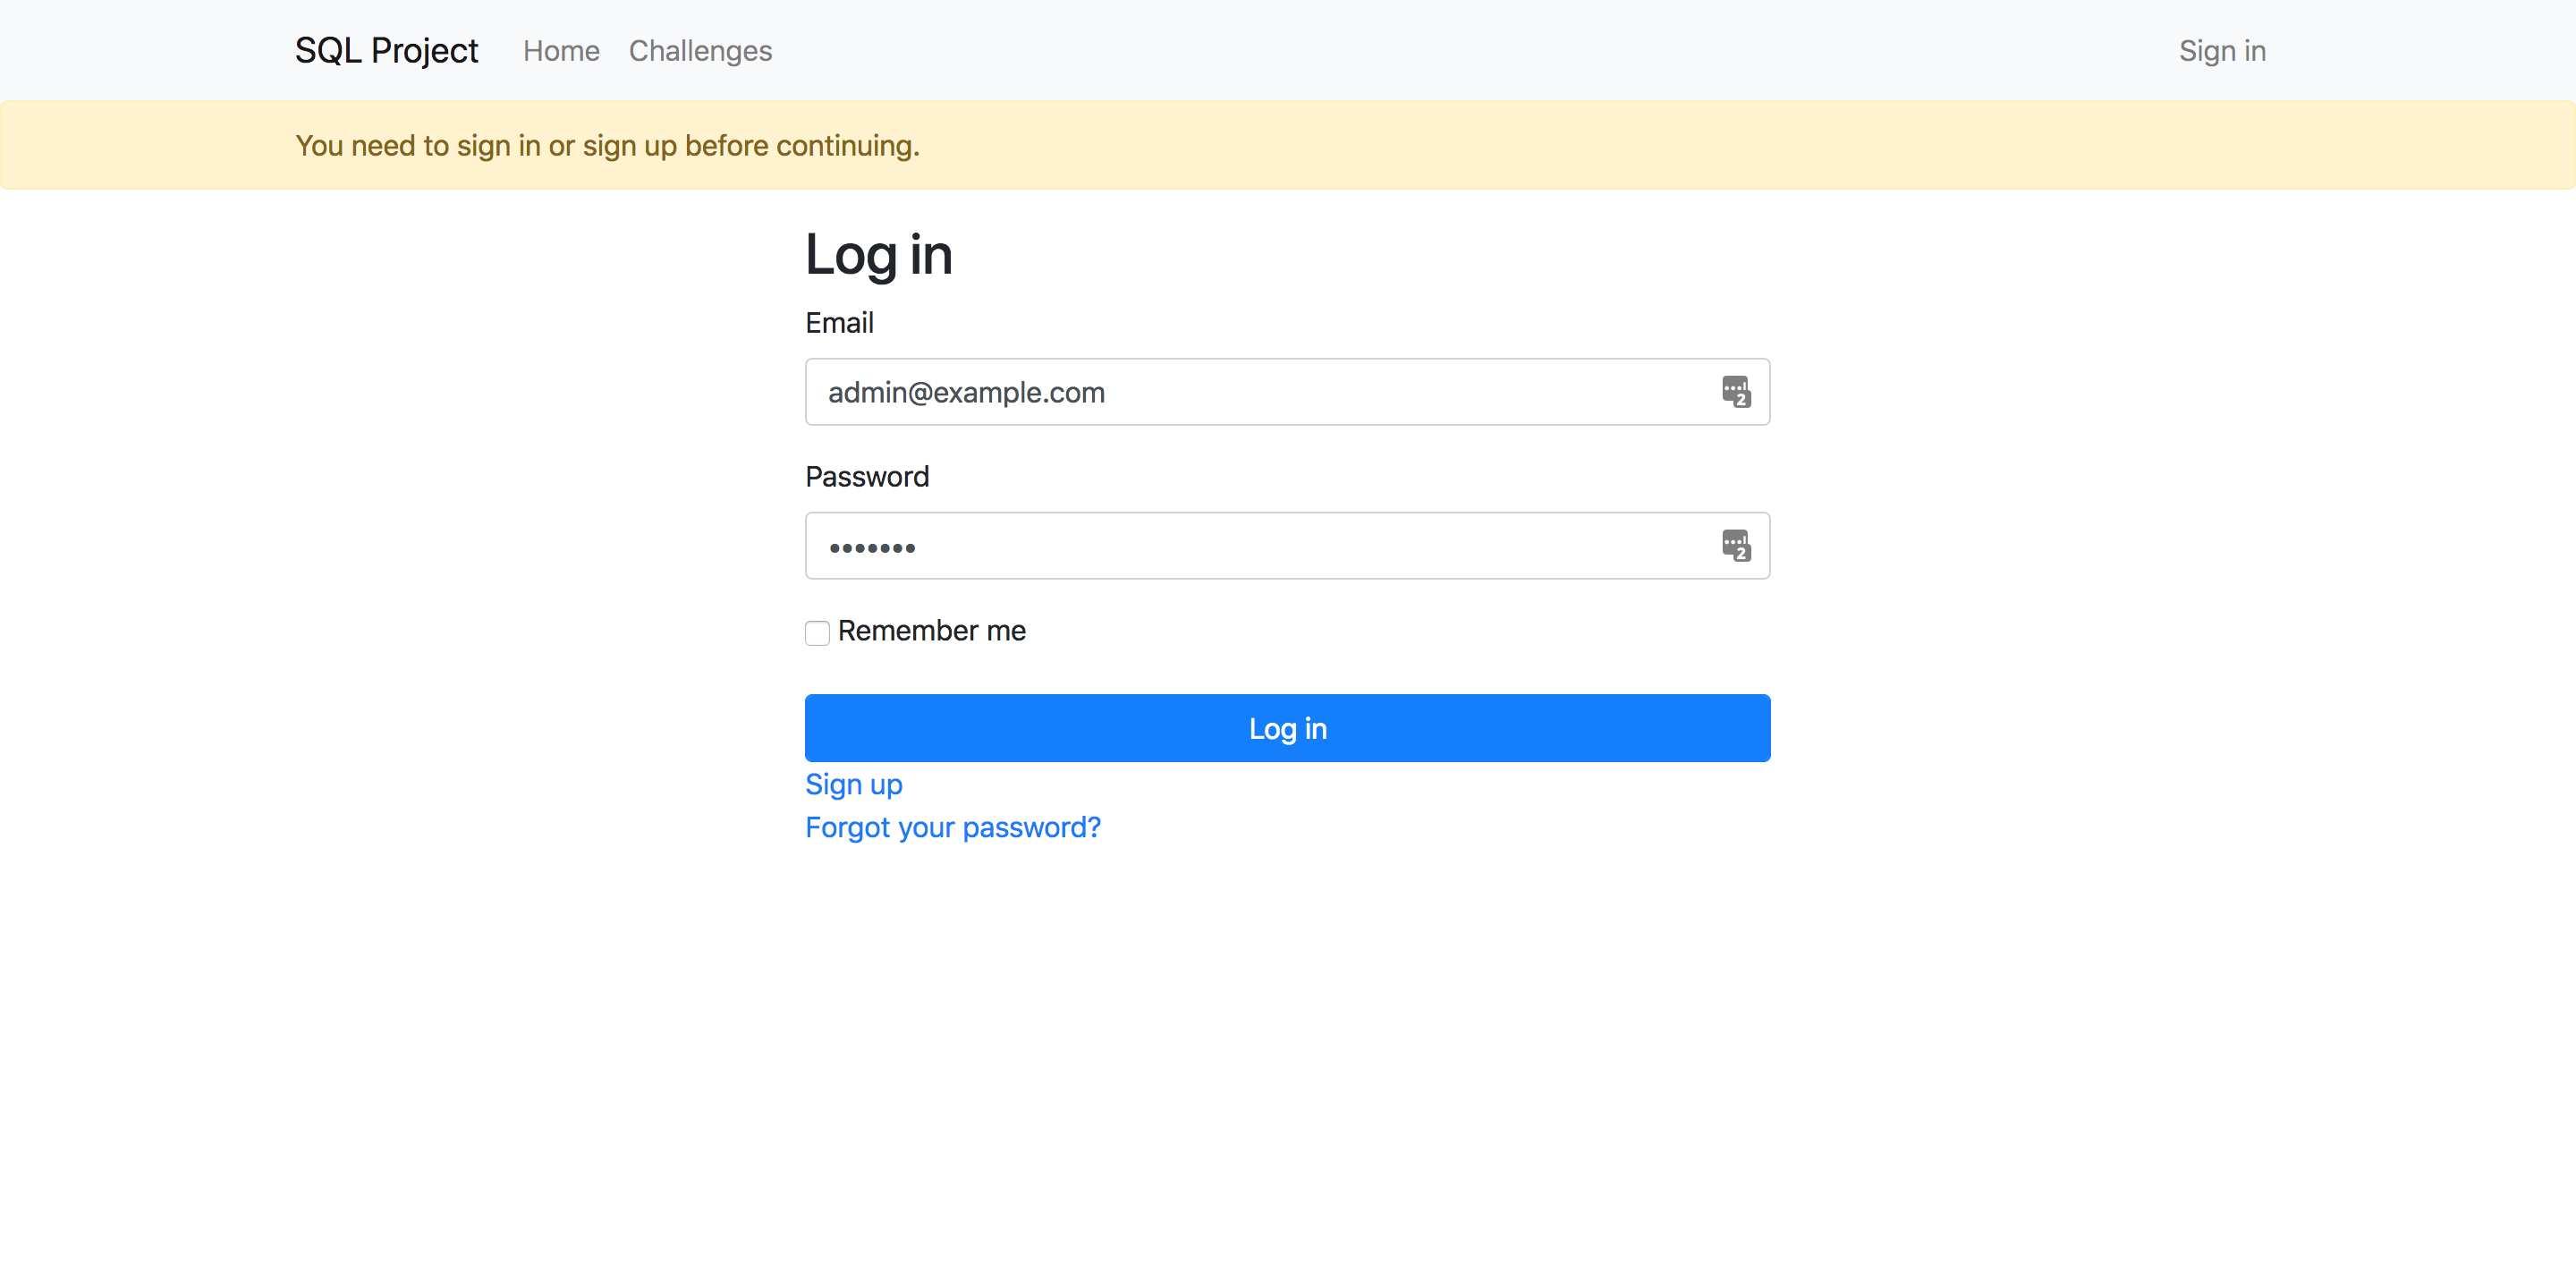
\includegraphics[width=\textwidth/4*3]{Appendices/authentication.png}
    \caption{Authentication screen}
    \label{fig:app:authentication}
\end{figure}

\Oldsubsection{Creating new user}
A new user can be created on the web application on path \texttt{/users/sign\_up} or by clicking the sing up button from the login page. Users are automatically marked as students. If a user uses a wrong email or password combination, he will see an error. An example of the sign-up page with errors is presented in figure \ref{fig:app:newuser}.

\begin{figure}[ht]
    \centering
    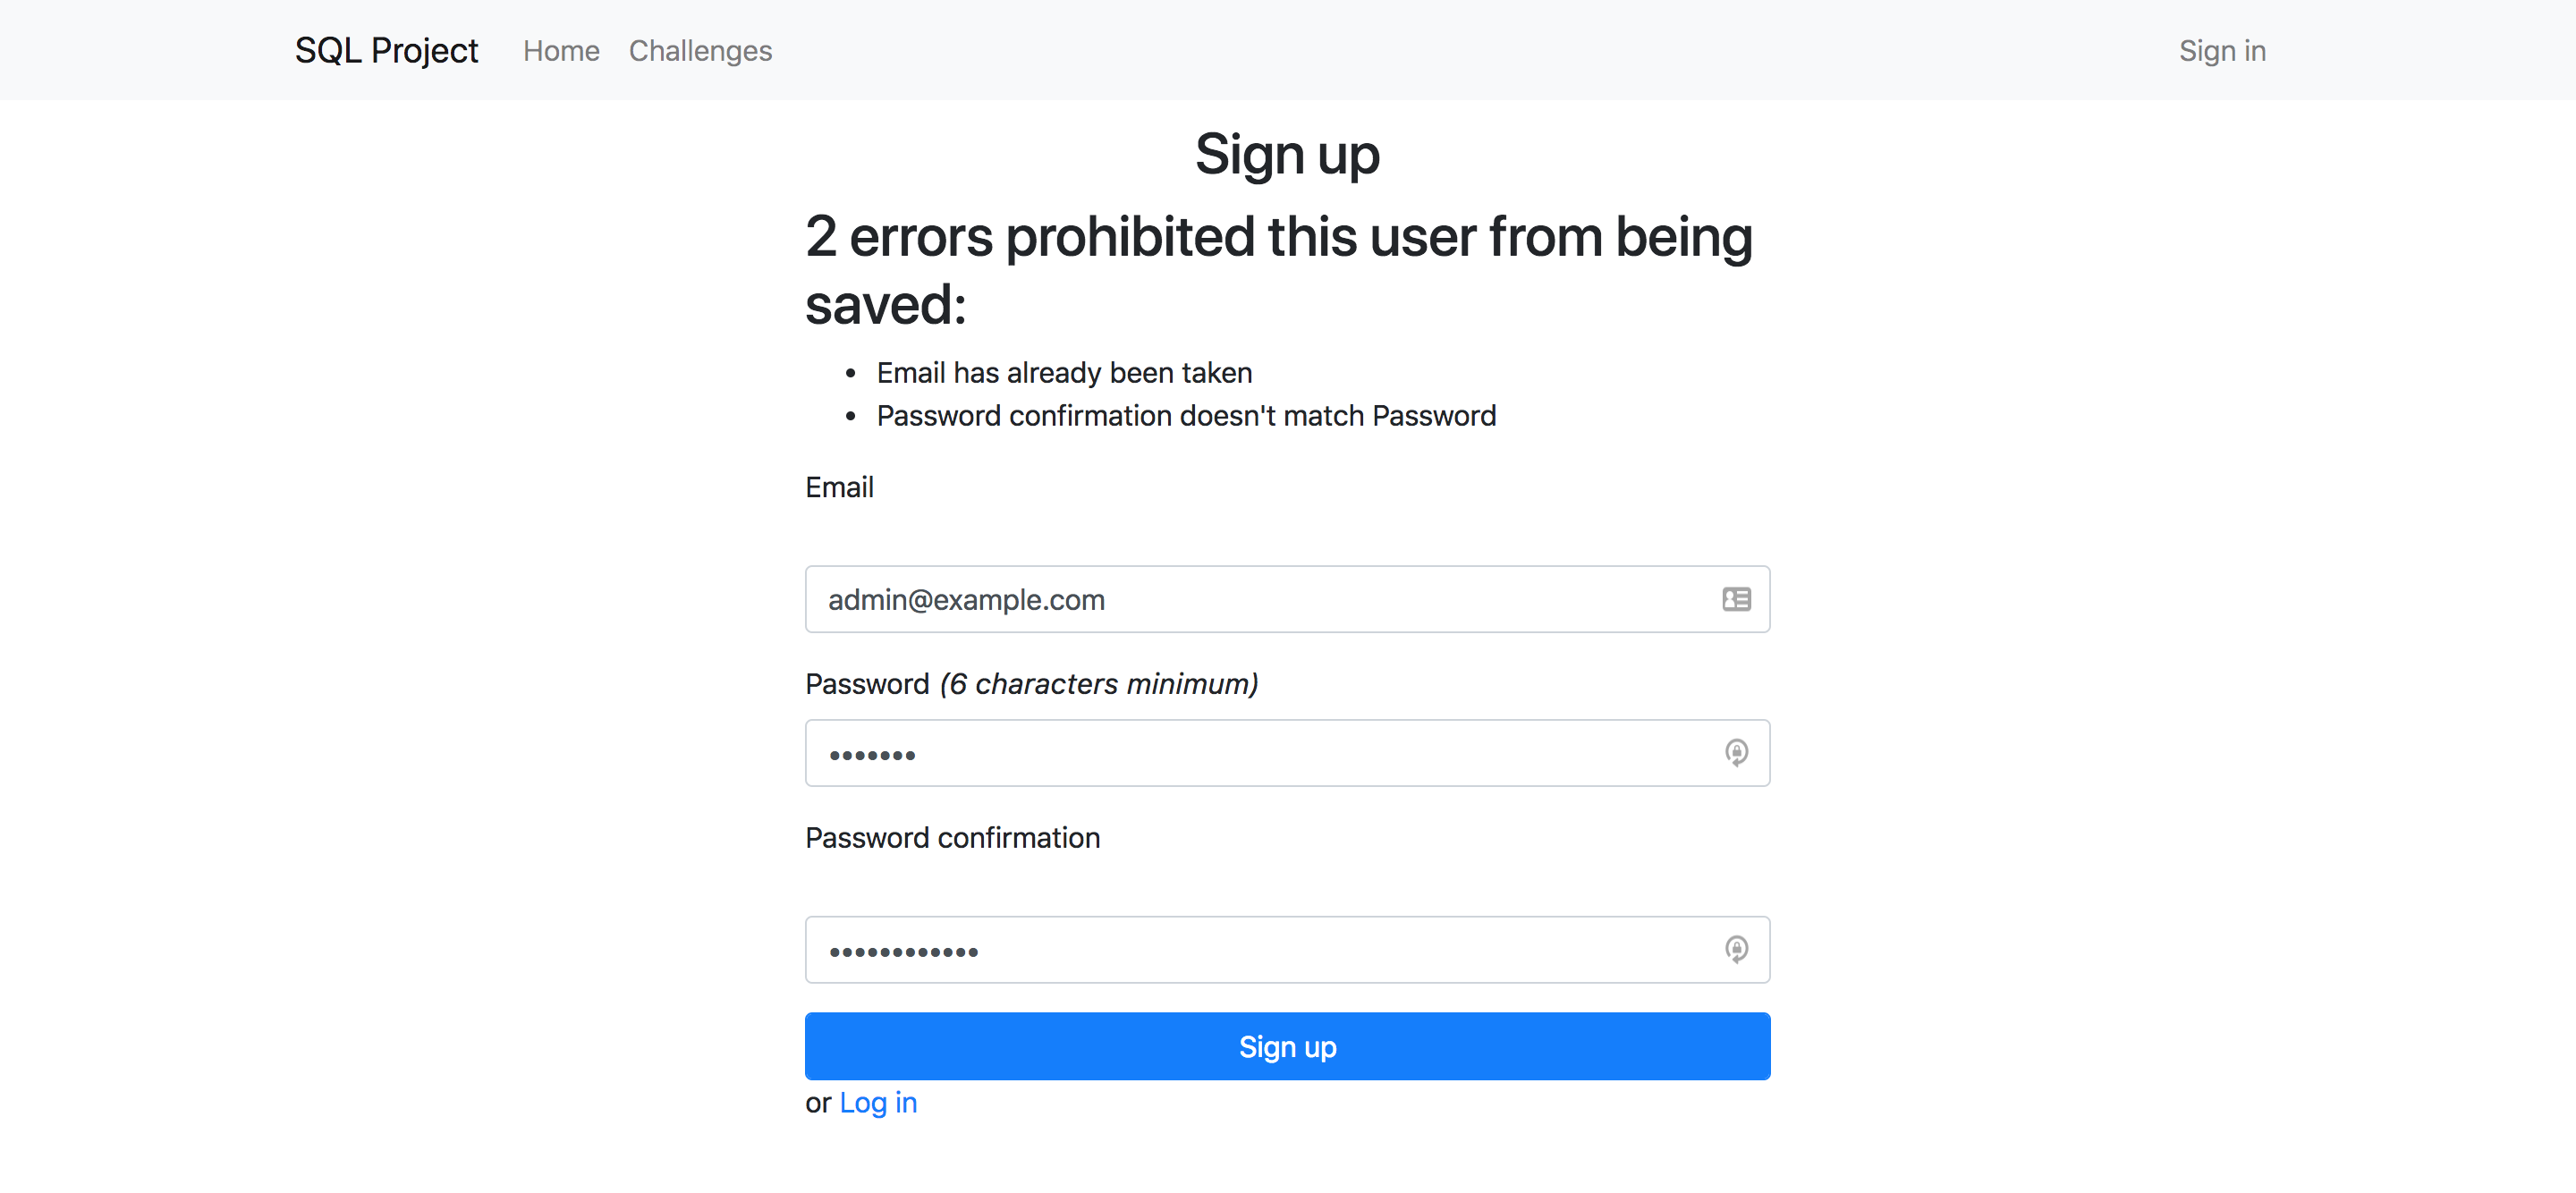
\includegraphics[width=\textwidth/4*3]{Appendices/signup.png}
    \caption{Sign-up screen}
    \label{fig:app:newuser}
\end{figure}

\Oldsubsection{Editing user details}
A user can change his details (email and password) on \texttt{/users/edit} or by clicking the Edit Profile in the navigation bar. The navigation bar link is presented in figure \ref{fig:app:editusernavbar} On this page, he can also delete his account. A photo of the page is included in figure \ref{fig:app:edituser}.

\begin{figure}[ht]
    \centering
    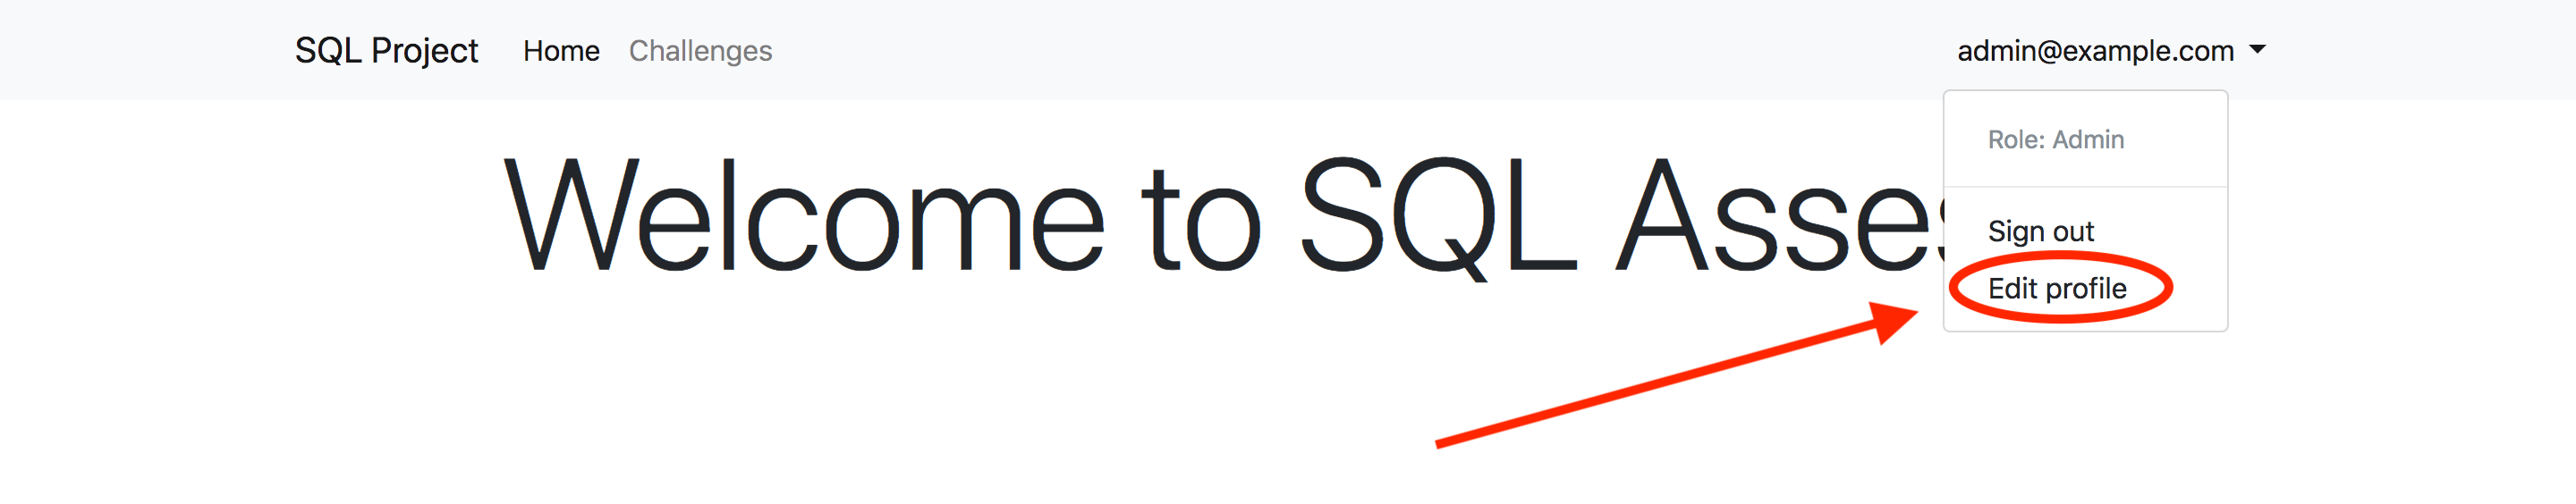
\includegraphics[width=\textwidth/4*3]{Appendices/editlinknavbar.png}
    \caption{Navigation bar link for edit user}
    \label{fig:app:editusernavbar}
\end{figure}

\begin{figure}[ht]
    \centering
    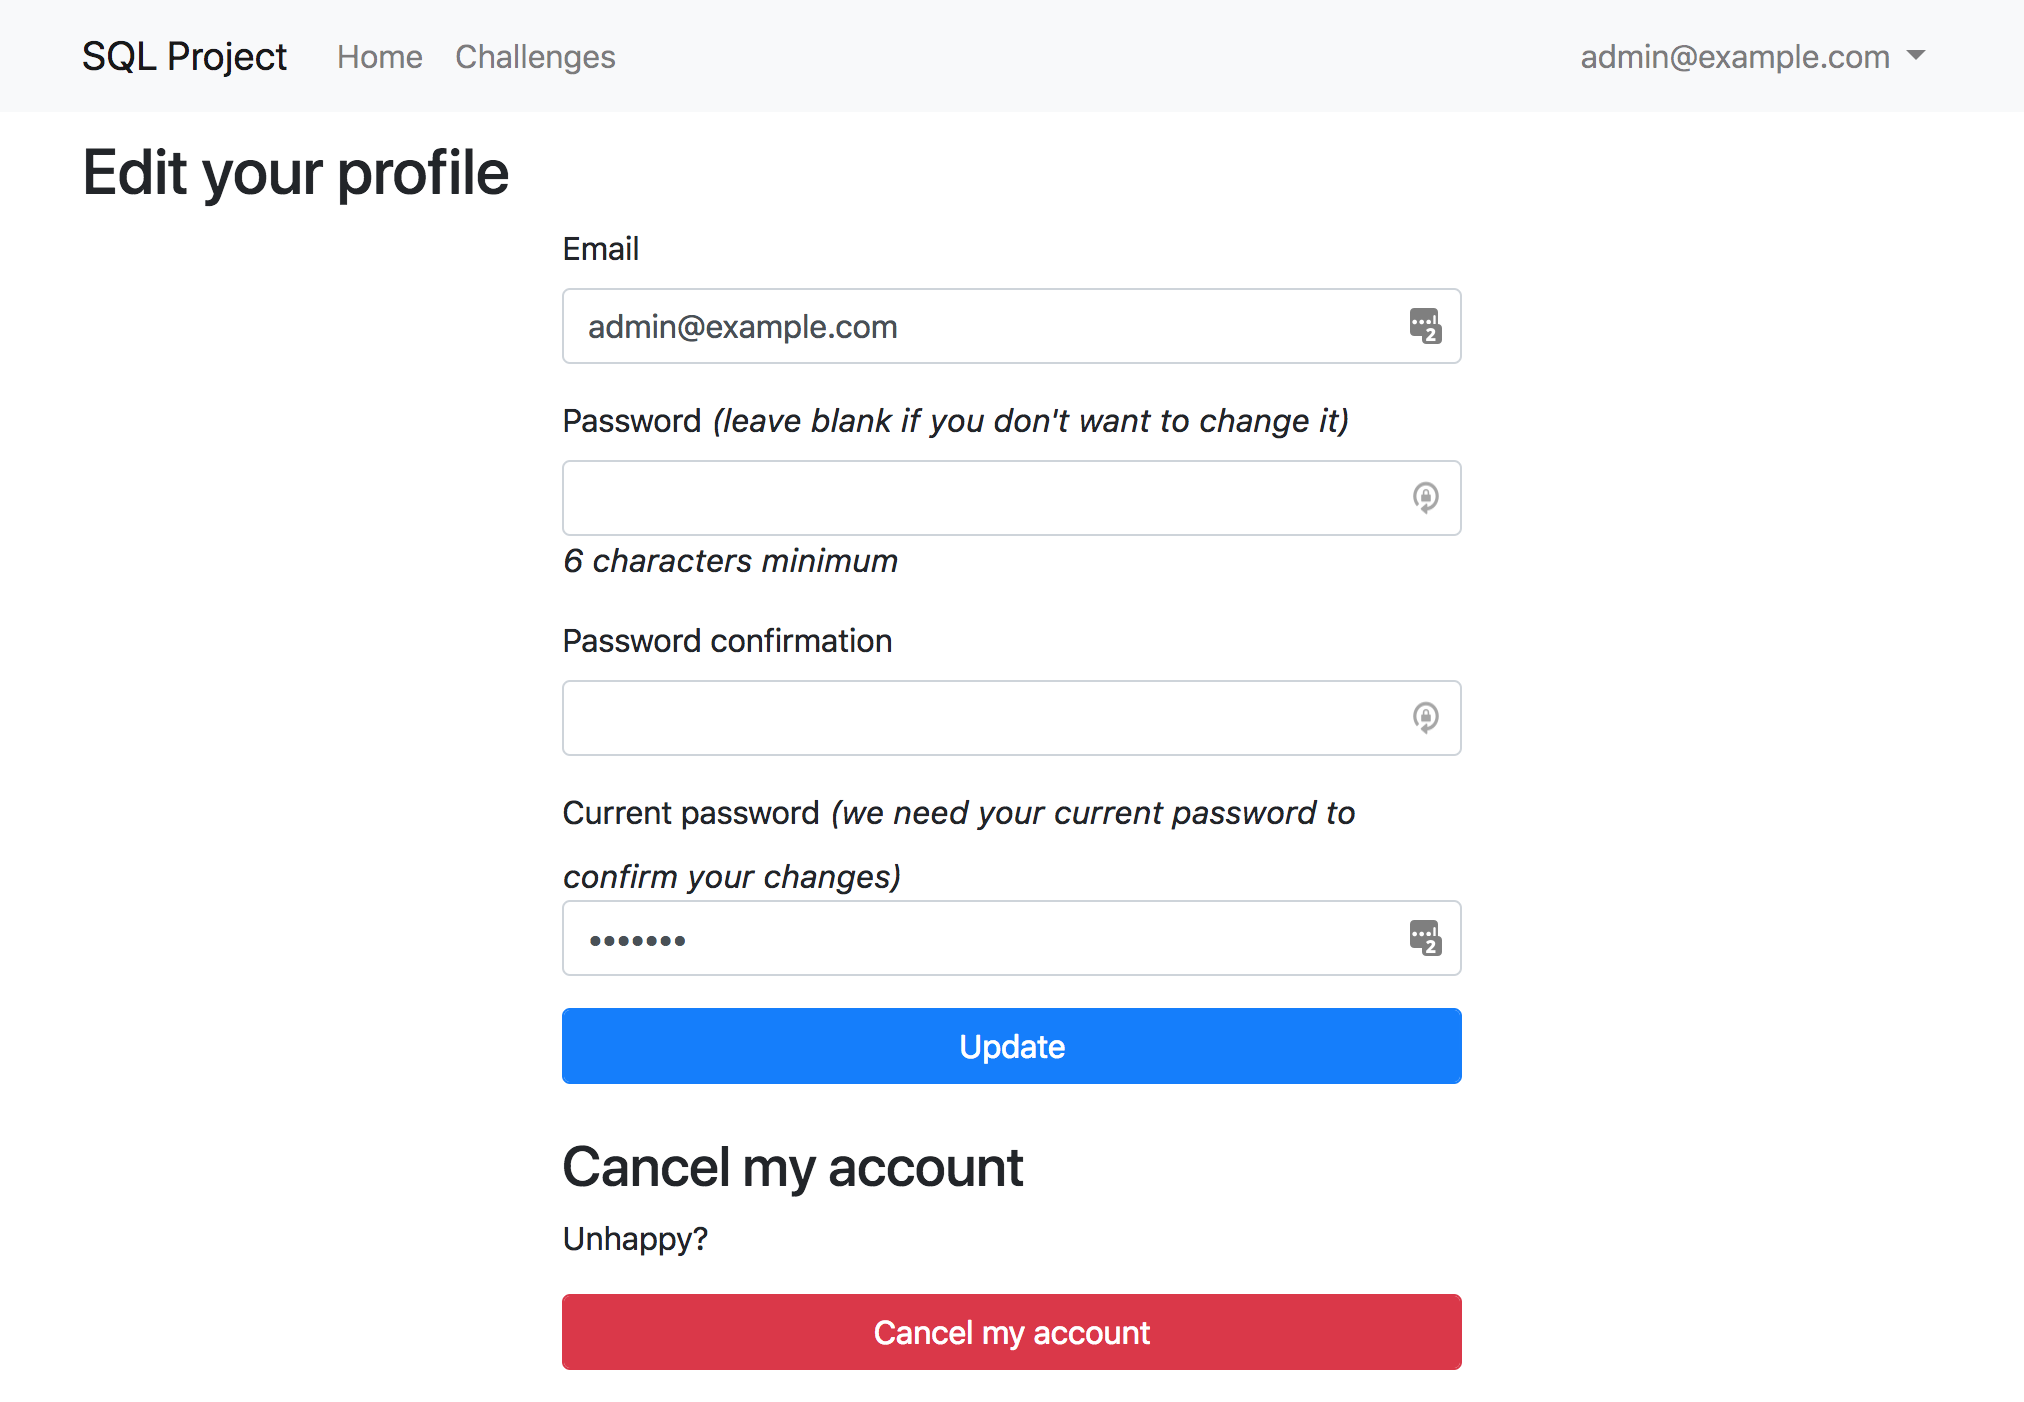
\includegraphics[width=\textwidth/4*3]{Appendices/edituser.png}
    \caption{Edit user page}
    \label{fig:app:edituser}
\end{figure}

\Oldsubsection{Sign-out}
Signing out is done from the navigation bar. Figure \ref{fig:app:signout} presents the location of the button.

\begin{figure}[ht]
    \centering
    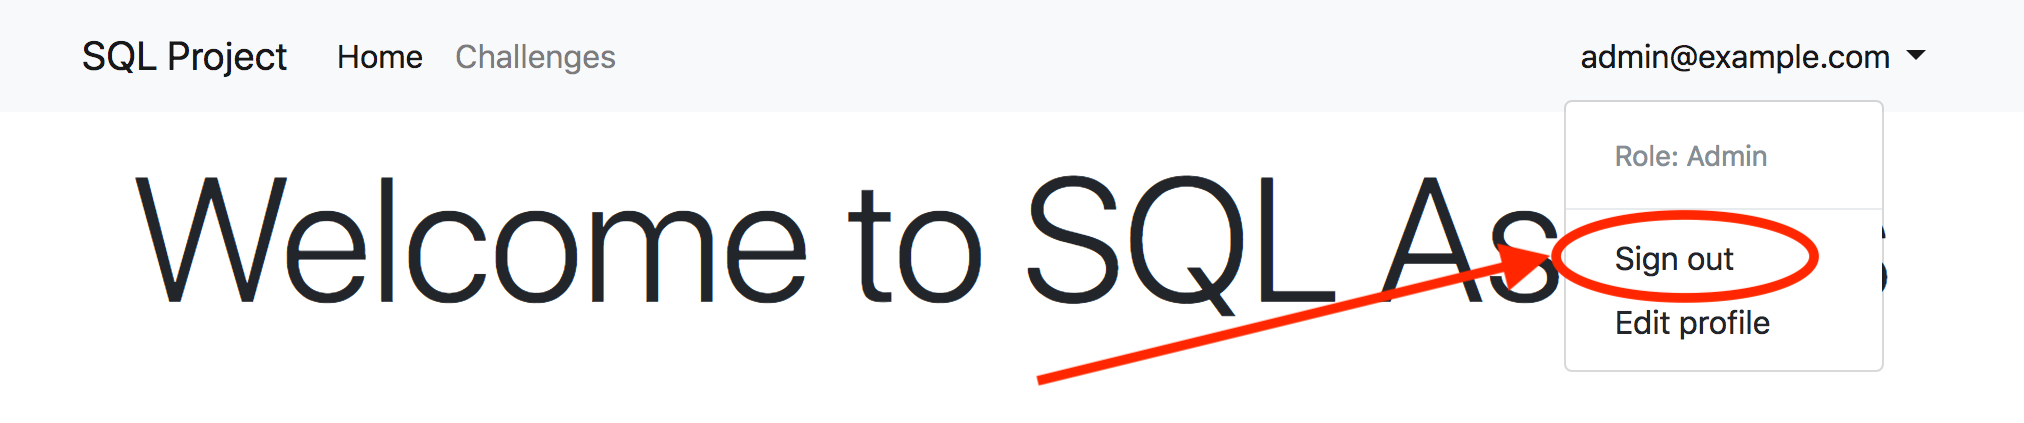
\includegraphics[width=\textwidth/4*3]{Appendices/signout.png}
    \caption{Sign out button}
    \label{fig:app:signout}
\end{figure}

\section{Challenge management}
To create a challenge, the current user must be an admin. To create a challenge, one must go to \texttt{/challenges/new}, or click \textit{Challenges} in the navigation bar, and then click \textit{Create new Challenge} button. The screen is presented in figure \ref{fig:app:new_challenge}.

The new challenge page requires 5 pieces of information:
\begin{enumerate}
    \item A title for the challenge
    \item The content or the challenge - or the body of the challenge
    \item SQL query for schema creation
    \item SQL query for data insertion
    \item The correct SQL query for the challenge
\end{enumerate}

The input for the SQL fields is a code editor that provides code syntax highlighting.

Any errors that might be encountered are shown to the user.
\begin{figure}[ht]
    \centering
    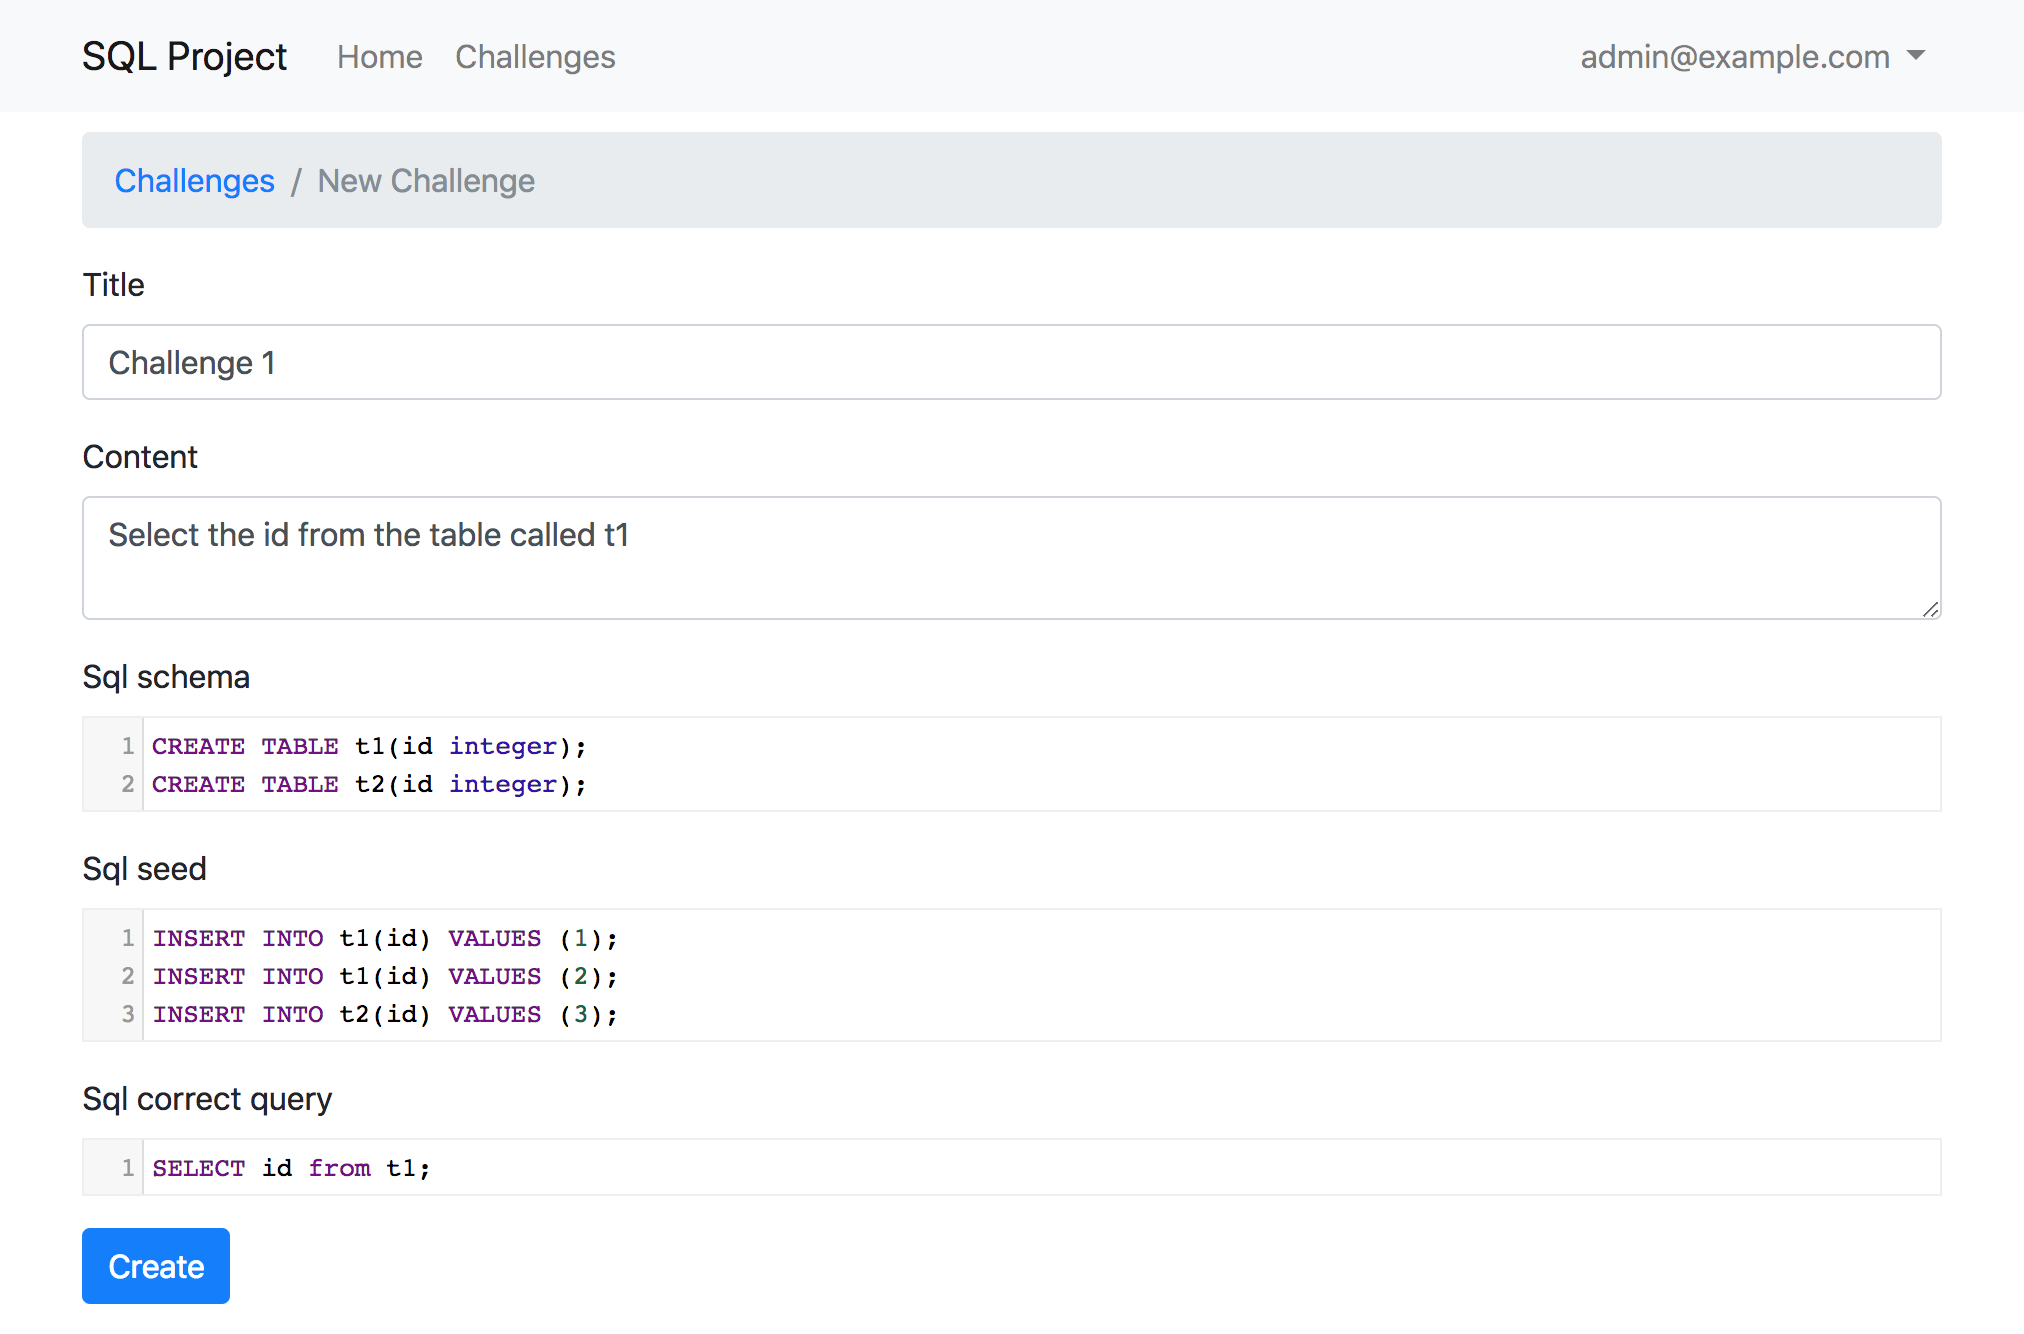
\includegraphics[width=\textwidth/4*3]{Appendices/new_challenge.png}
    \caption{New challenge form}
    \label{fig:app:new_challenge}
\end{figure}

Once the challenge has been saved, the user is redirect to the challenge page which contains all the details about the challenge (schema and existing fields). A screen-shot of the page is show in figure \ref{fig:app:challengeadmin}.

\begin{figure}[ht]
    \centering
    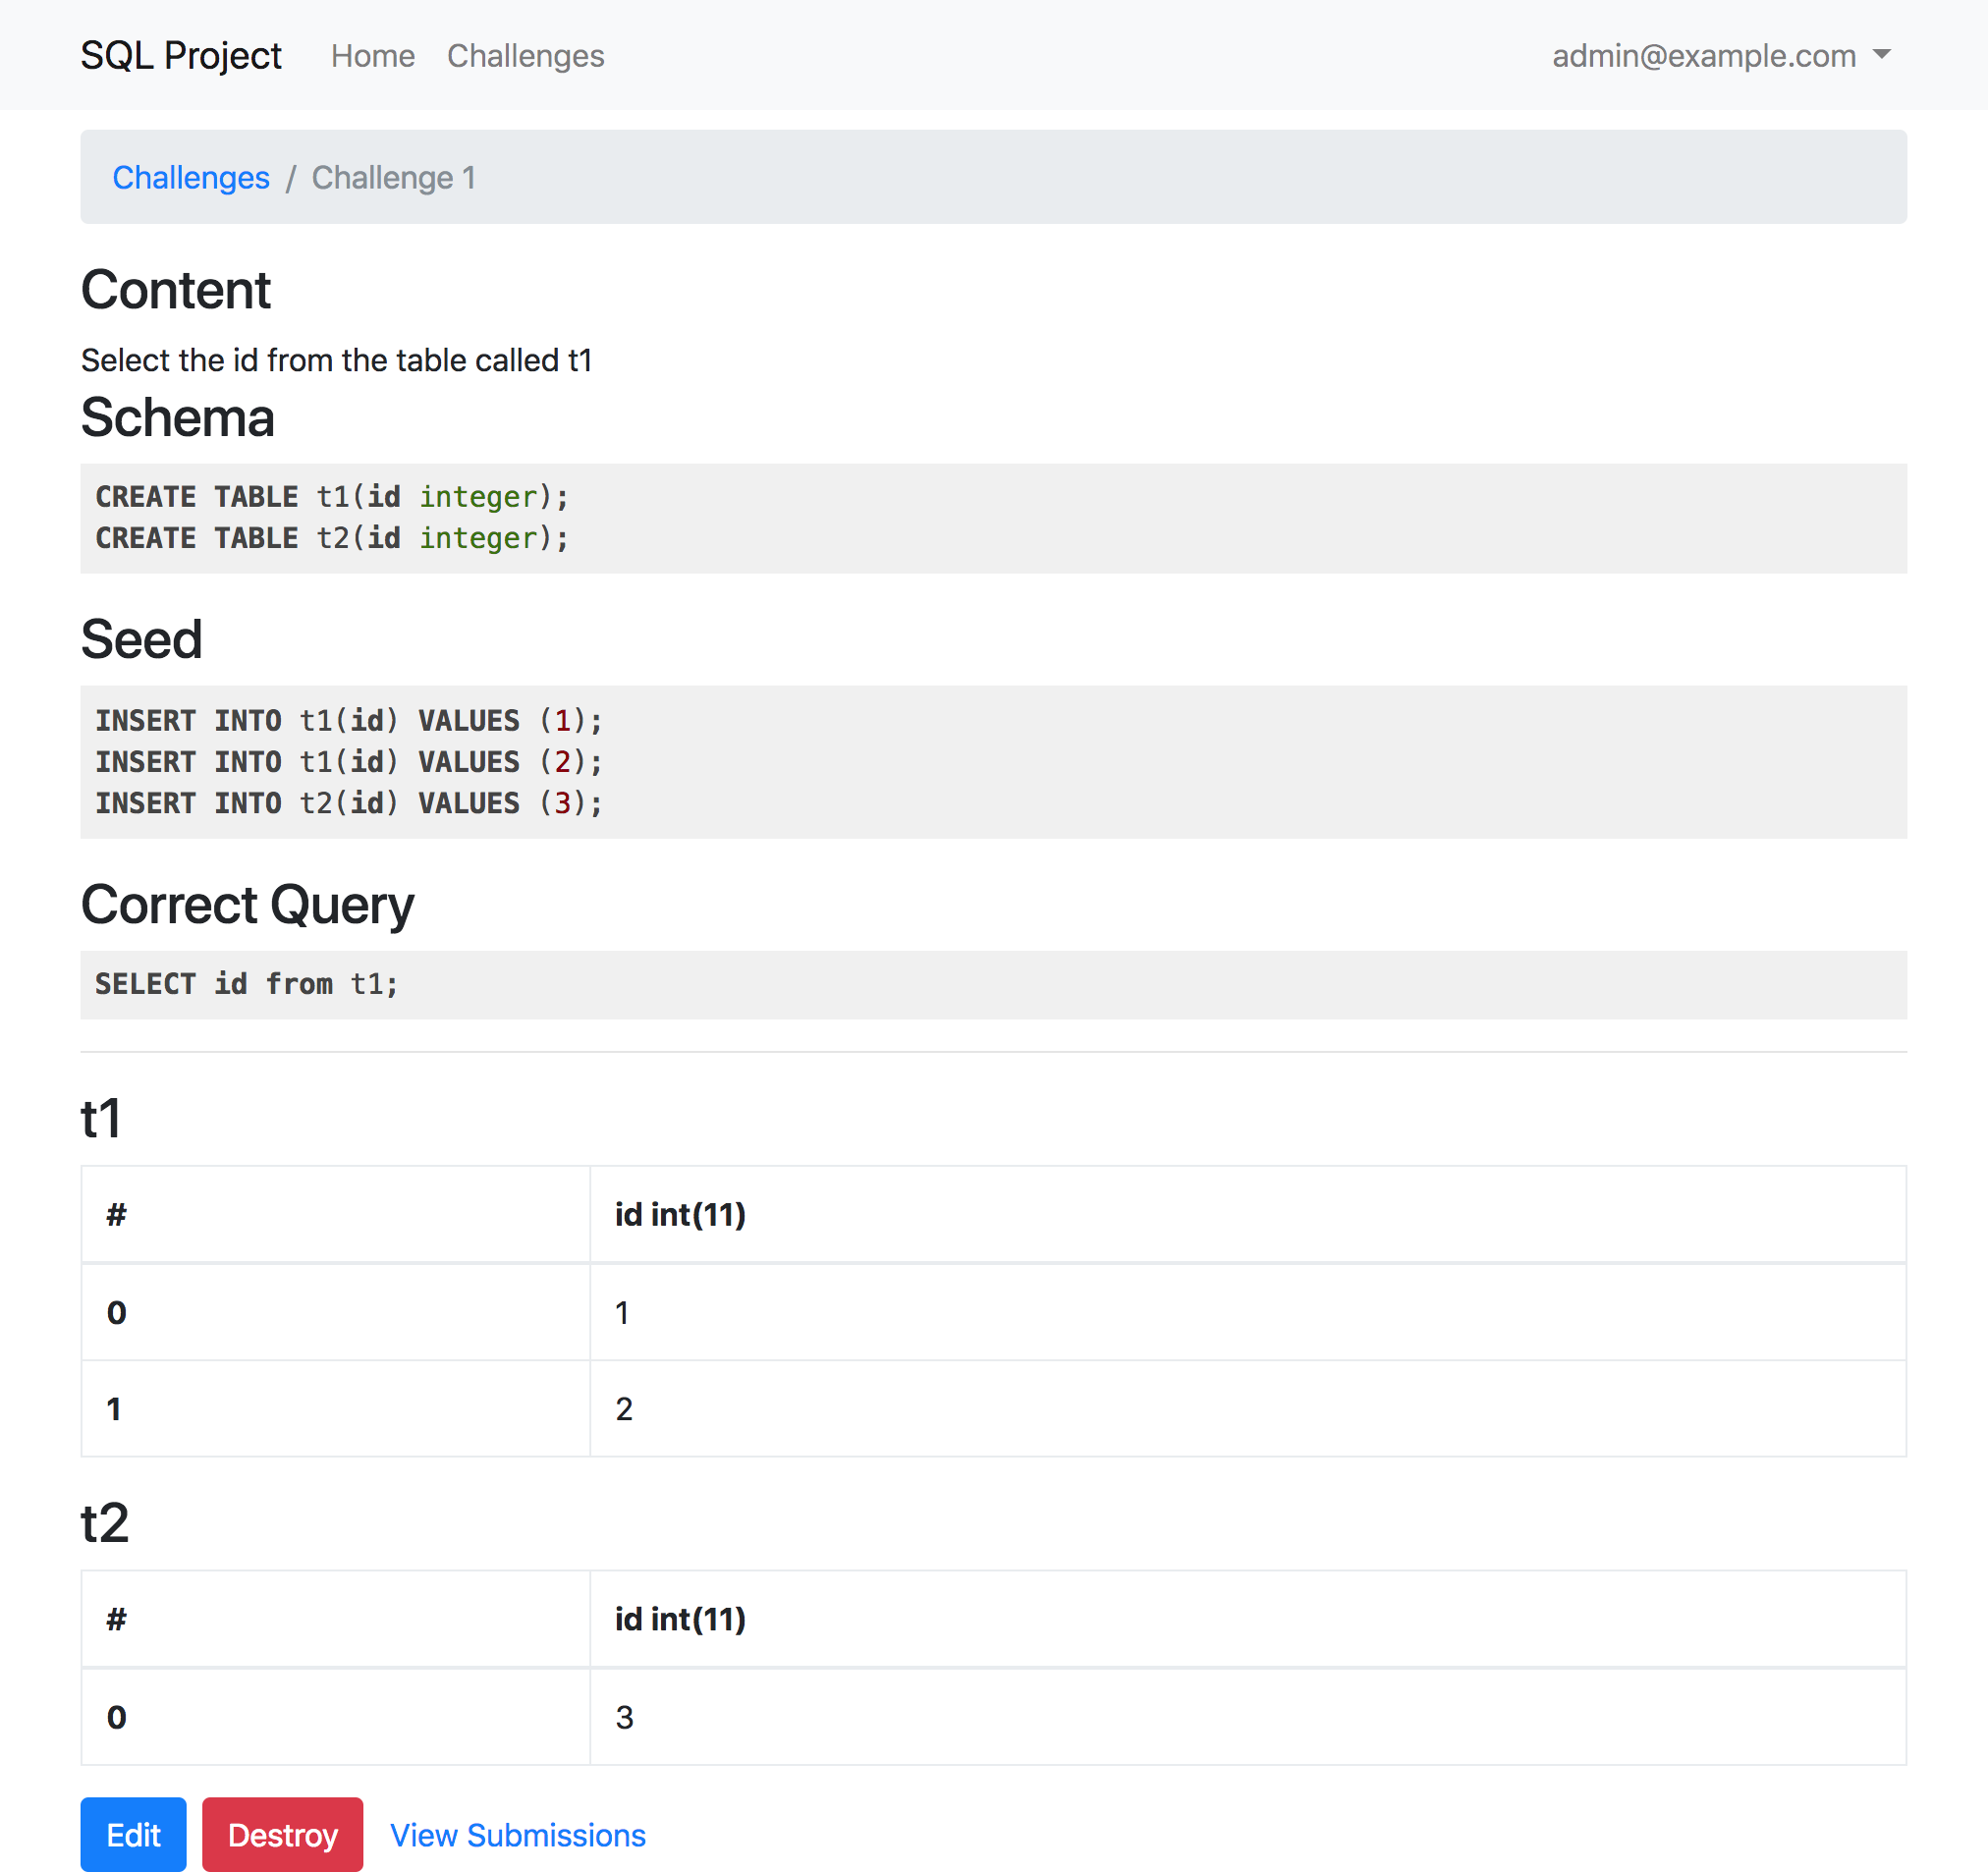
\includegraphics[width=\textwidth/4*3]{Appendices/adminchallenge.png}
    \caption{Admin's view of a new challenge}
    \label{fig:app:challengeadmin}
\end{figure}

An admin can then edit any challenge by clicking the edit button at the bottom of the page \ref{fig:app:challengeadmin}. The edit page is very similar to the creation form (\ref{fig:app:new_challenge}).

An admin can also delete a challenge by clicking the Destroy button at the bottom of the page \ref{fig:app:challengeadmin}.

\section{Submissions: student's view}

A student can submit a solution by first going to the \textit{New submission page}. To go to that page, he first needs to visit the challenges page (from the navigation bar), and then click the \textit{New submission} link for the desired challenge. The instructions are presented in figure \ref{fig:app:new_submission}.

\begin{figure}[ht]
    \centering
    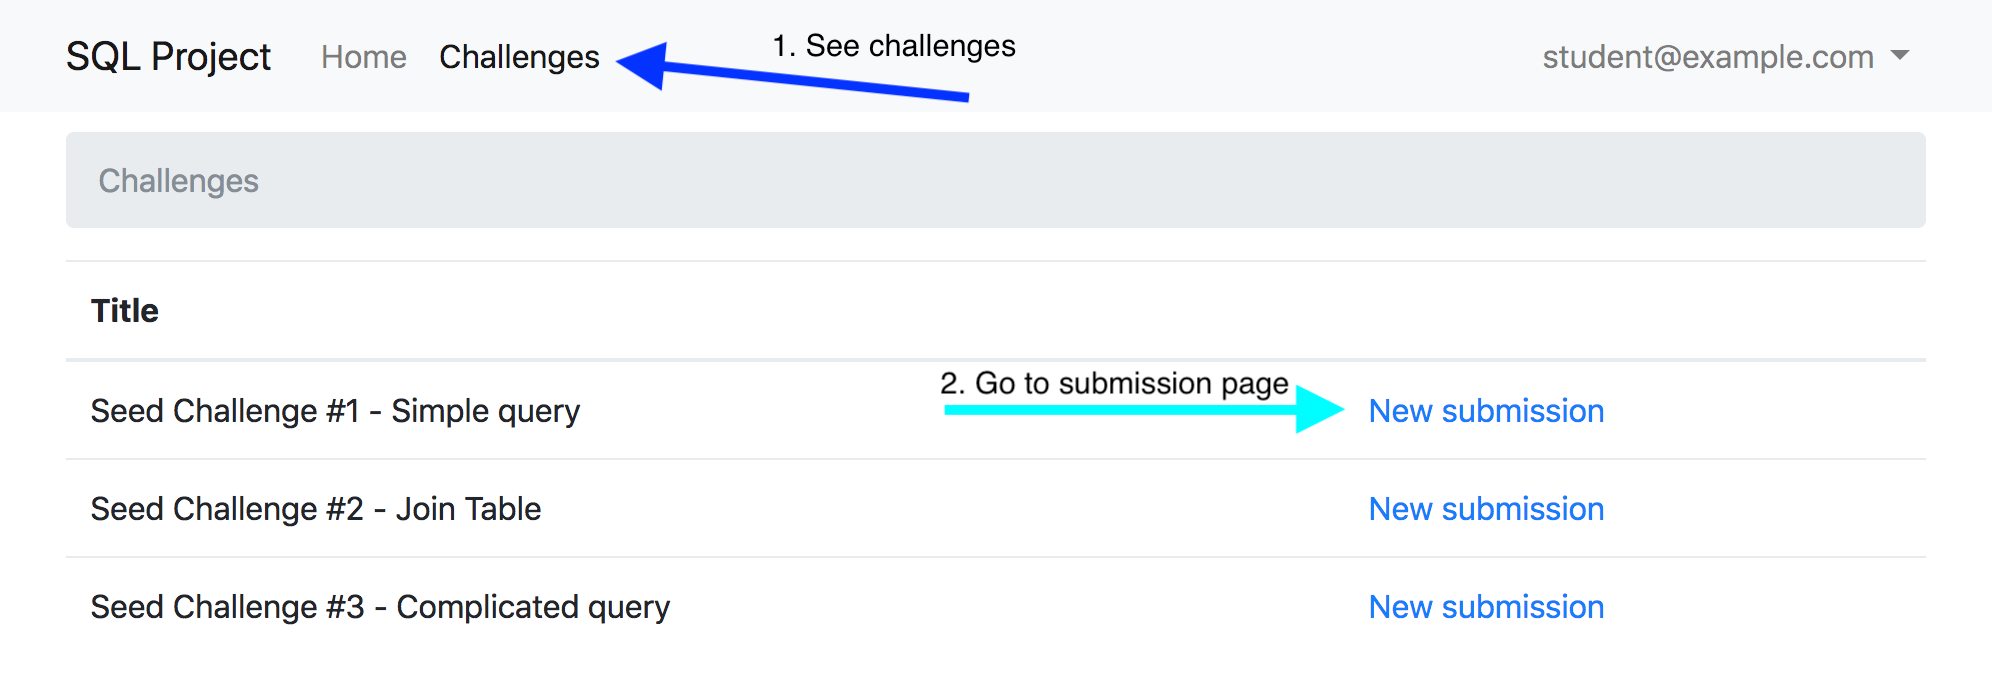
\includegraphics[width=\textwidth/4*3]{Appendices/challengeinde.png}
    \caption{Going to new submission page}
    \label{fig:app:new_submission}
\end{figure}

Once the user gets to that page, he will be able to see the schema of the database, both in the SQL form and in a tabular form. Here he can type the solution to the query. Figure \ref{fig:app:submit} presents this screen.

\begin{figure}[ht]
    \centering
    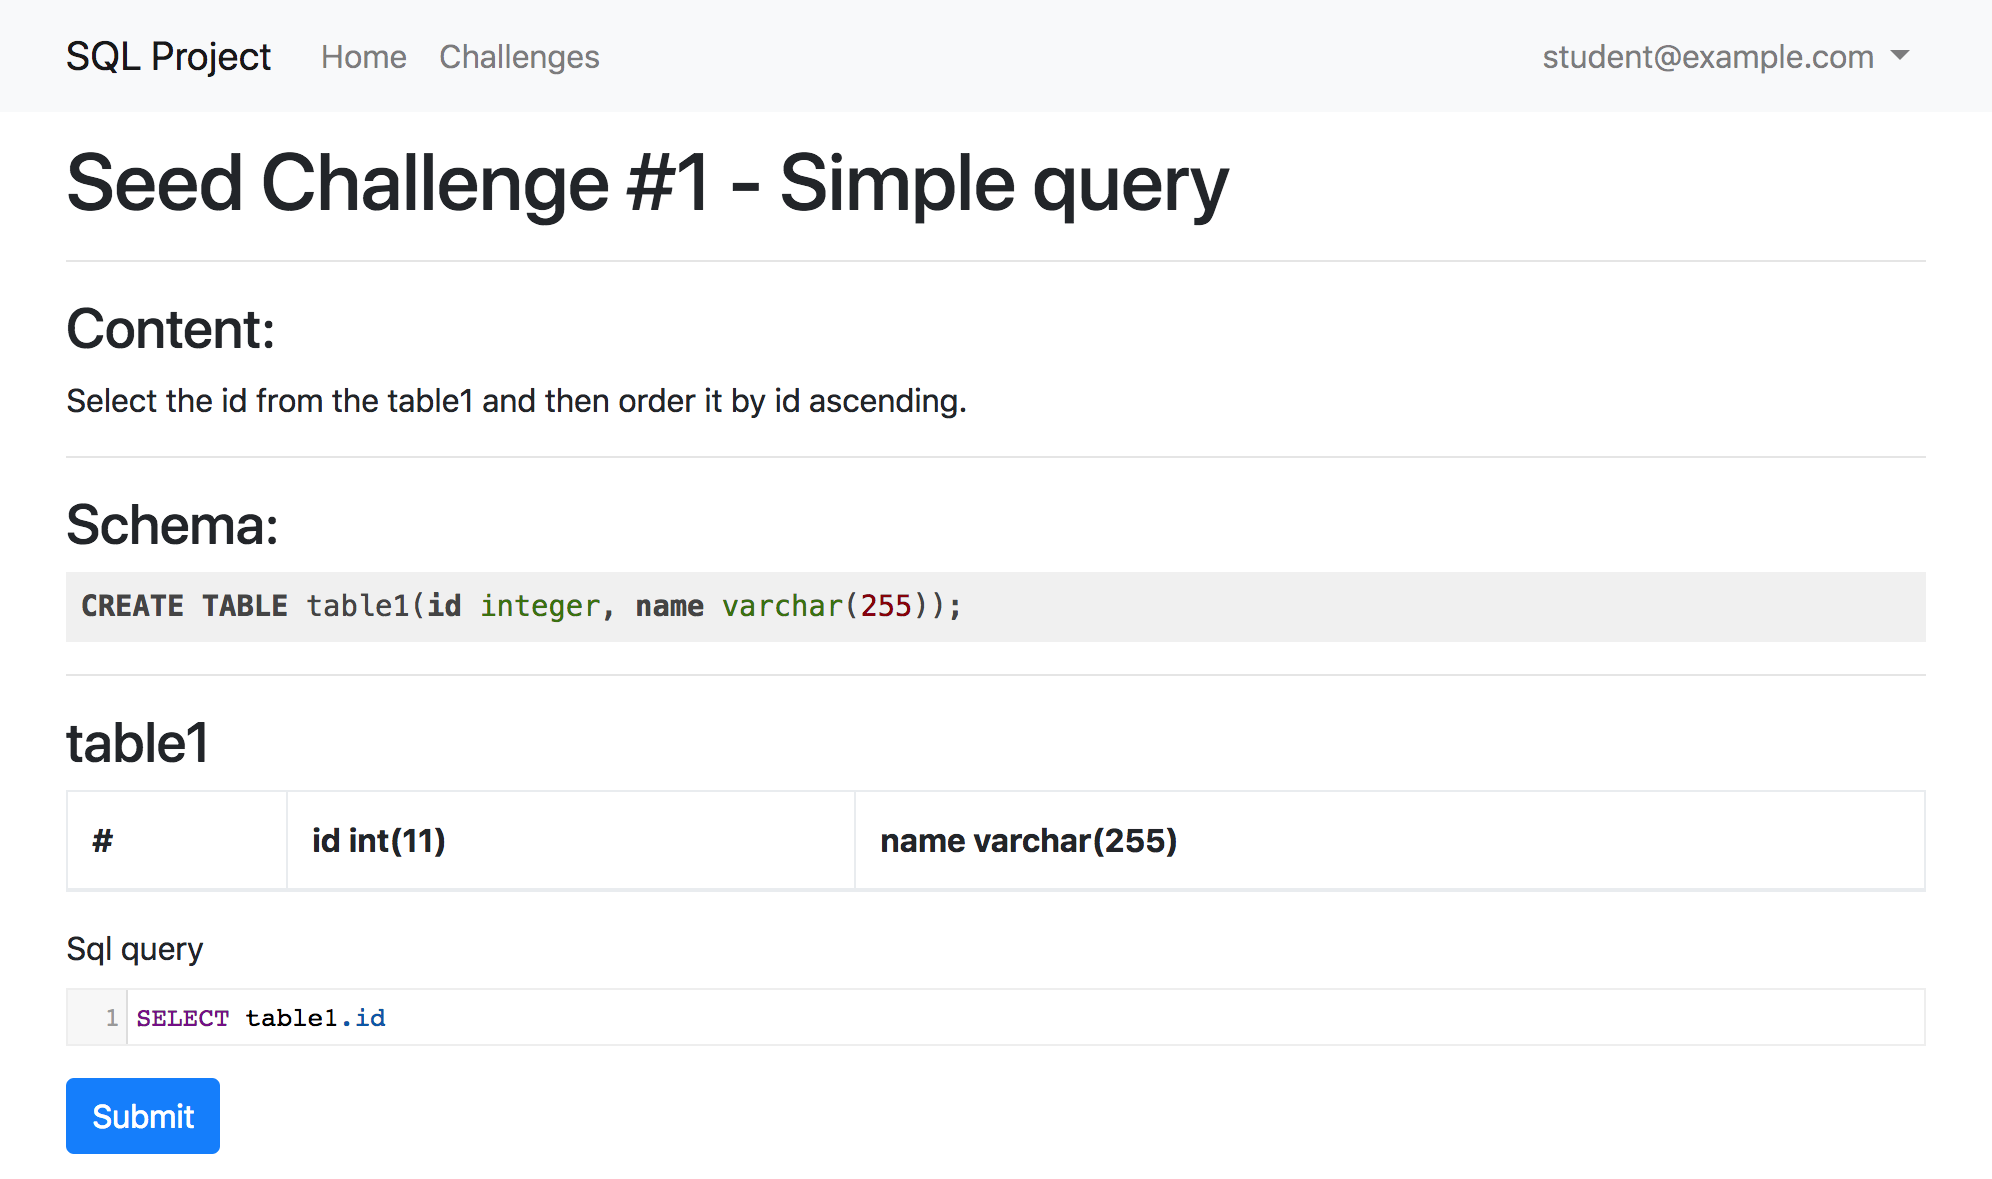
\includegraphics[width=\textwidth/4*3]{Appendices/submit.png}
    \caption{Submit solution page}
    \label{fig:app:submit}
\end{figure}

By clicking the Submit button on the page, the student will be able to see the results of the submission. If the query submitted has SQL errors, the user will see the errors on the same page (example in figure \ref{fig:app:submit_errors}.

\begin{figure}
    \centering
    
\includegraphics[width=\textwidth/4*3]{Appendices/submit_errors.png}
    \caption{Submit errors}
    \label{fig:app:submit_errors}
\end{figure}

If the compilation is successful, the user will either see a success message if the query is correct (figure \ref{fig:app:submit_correct}), or a hint if it's incorrect (figure \ref{fig:app:submit_incorrect}).

\begin{figure}[H]
    \centering
    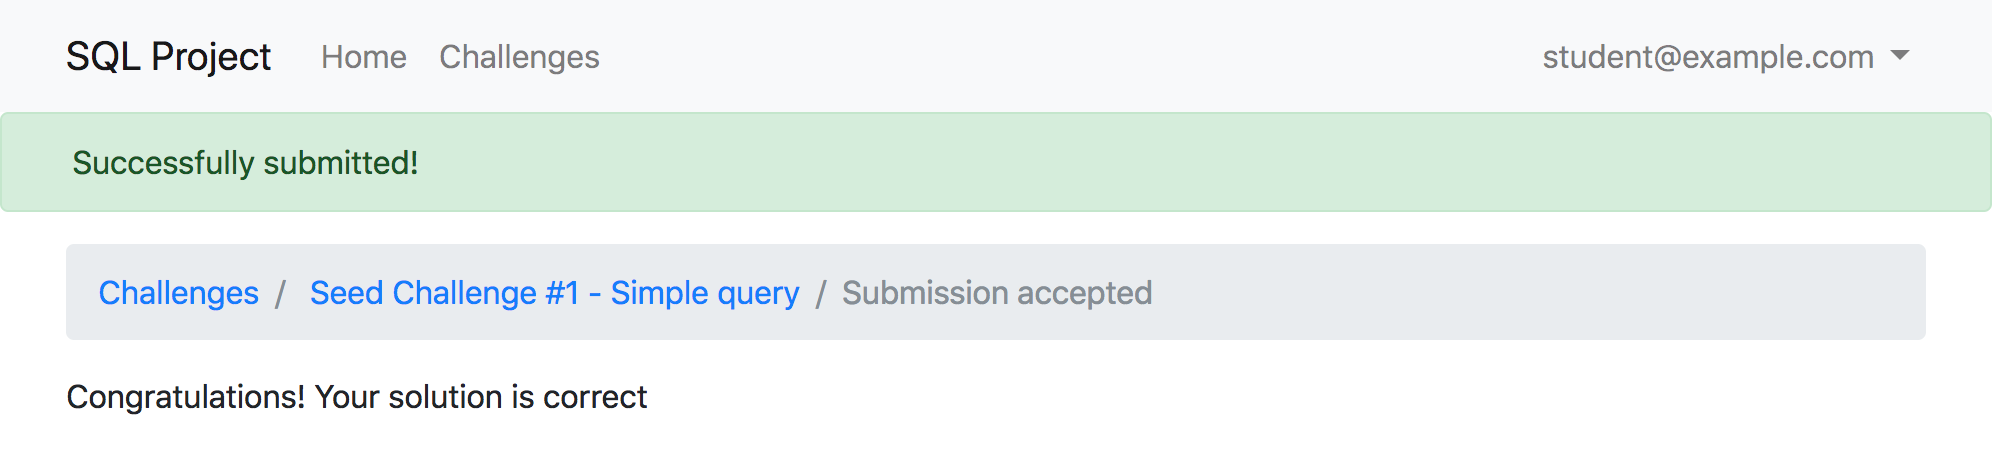
\includegraphics[width=\textwidth/4*3]{Appendices/submit_correct.png}
    \caption{Submission message for correct query}
    \label{fig:app:submit_correct}
\end{figure}

\begin{figure}[H]
    \centering
    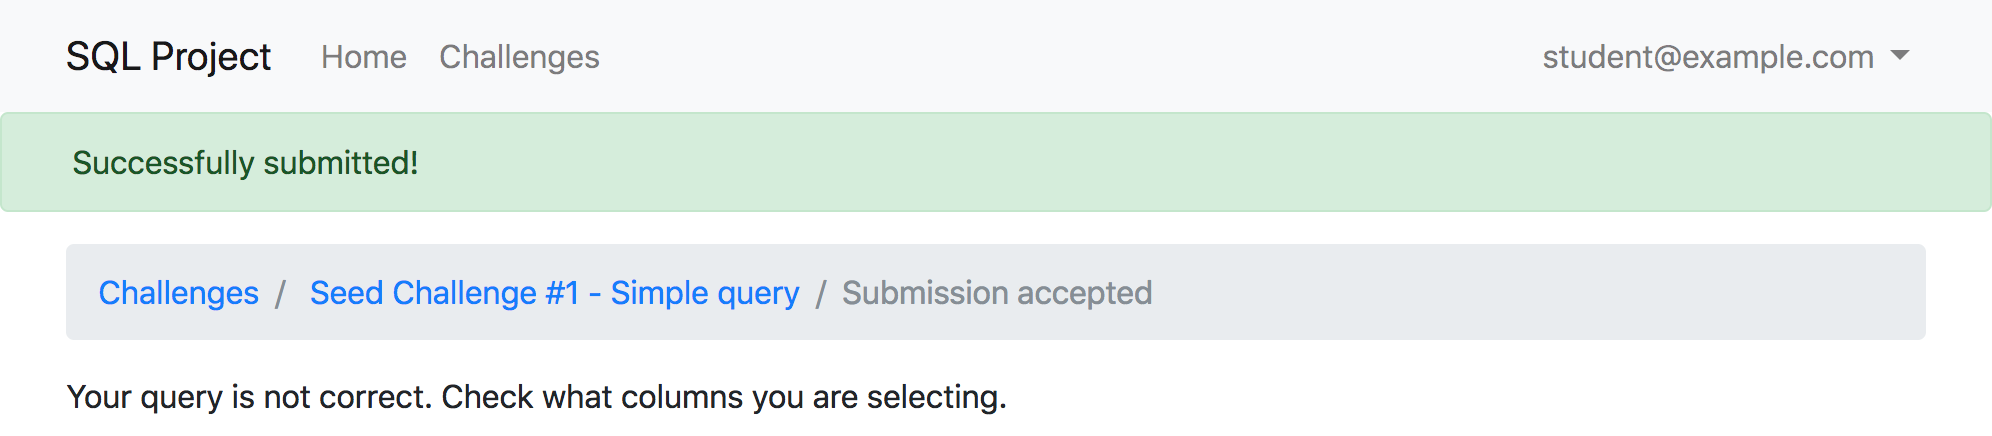
\includegraphics[width=\textwidth/4*3]{Appendices/submit_hint.png}
    \caption{Submission message for correct query}
    \label{fig:app:submit_incorrect}
\end{figure}

\section{Submissions: instructor's view}

To view student's submissions for a challenge, the instructor must click the link "View submissions" from the challenge page (presented in \ref{fig:app:challengeadmin}). The submissions page will include all submissions for a challenge. The page is presented in figure \ref{fig:app:submissions}.

\begin{figure}[ht]
    \centering
    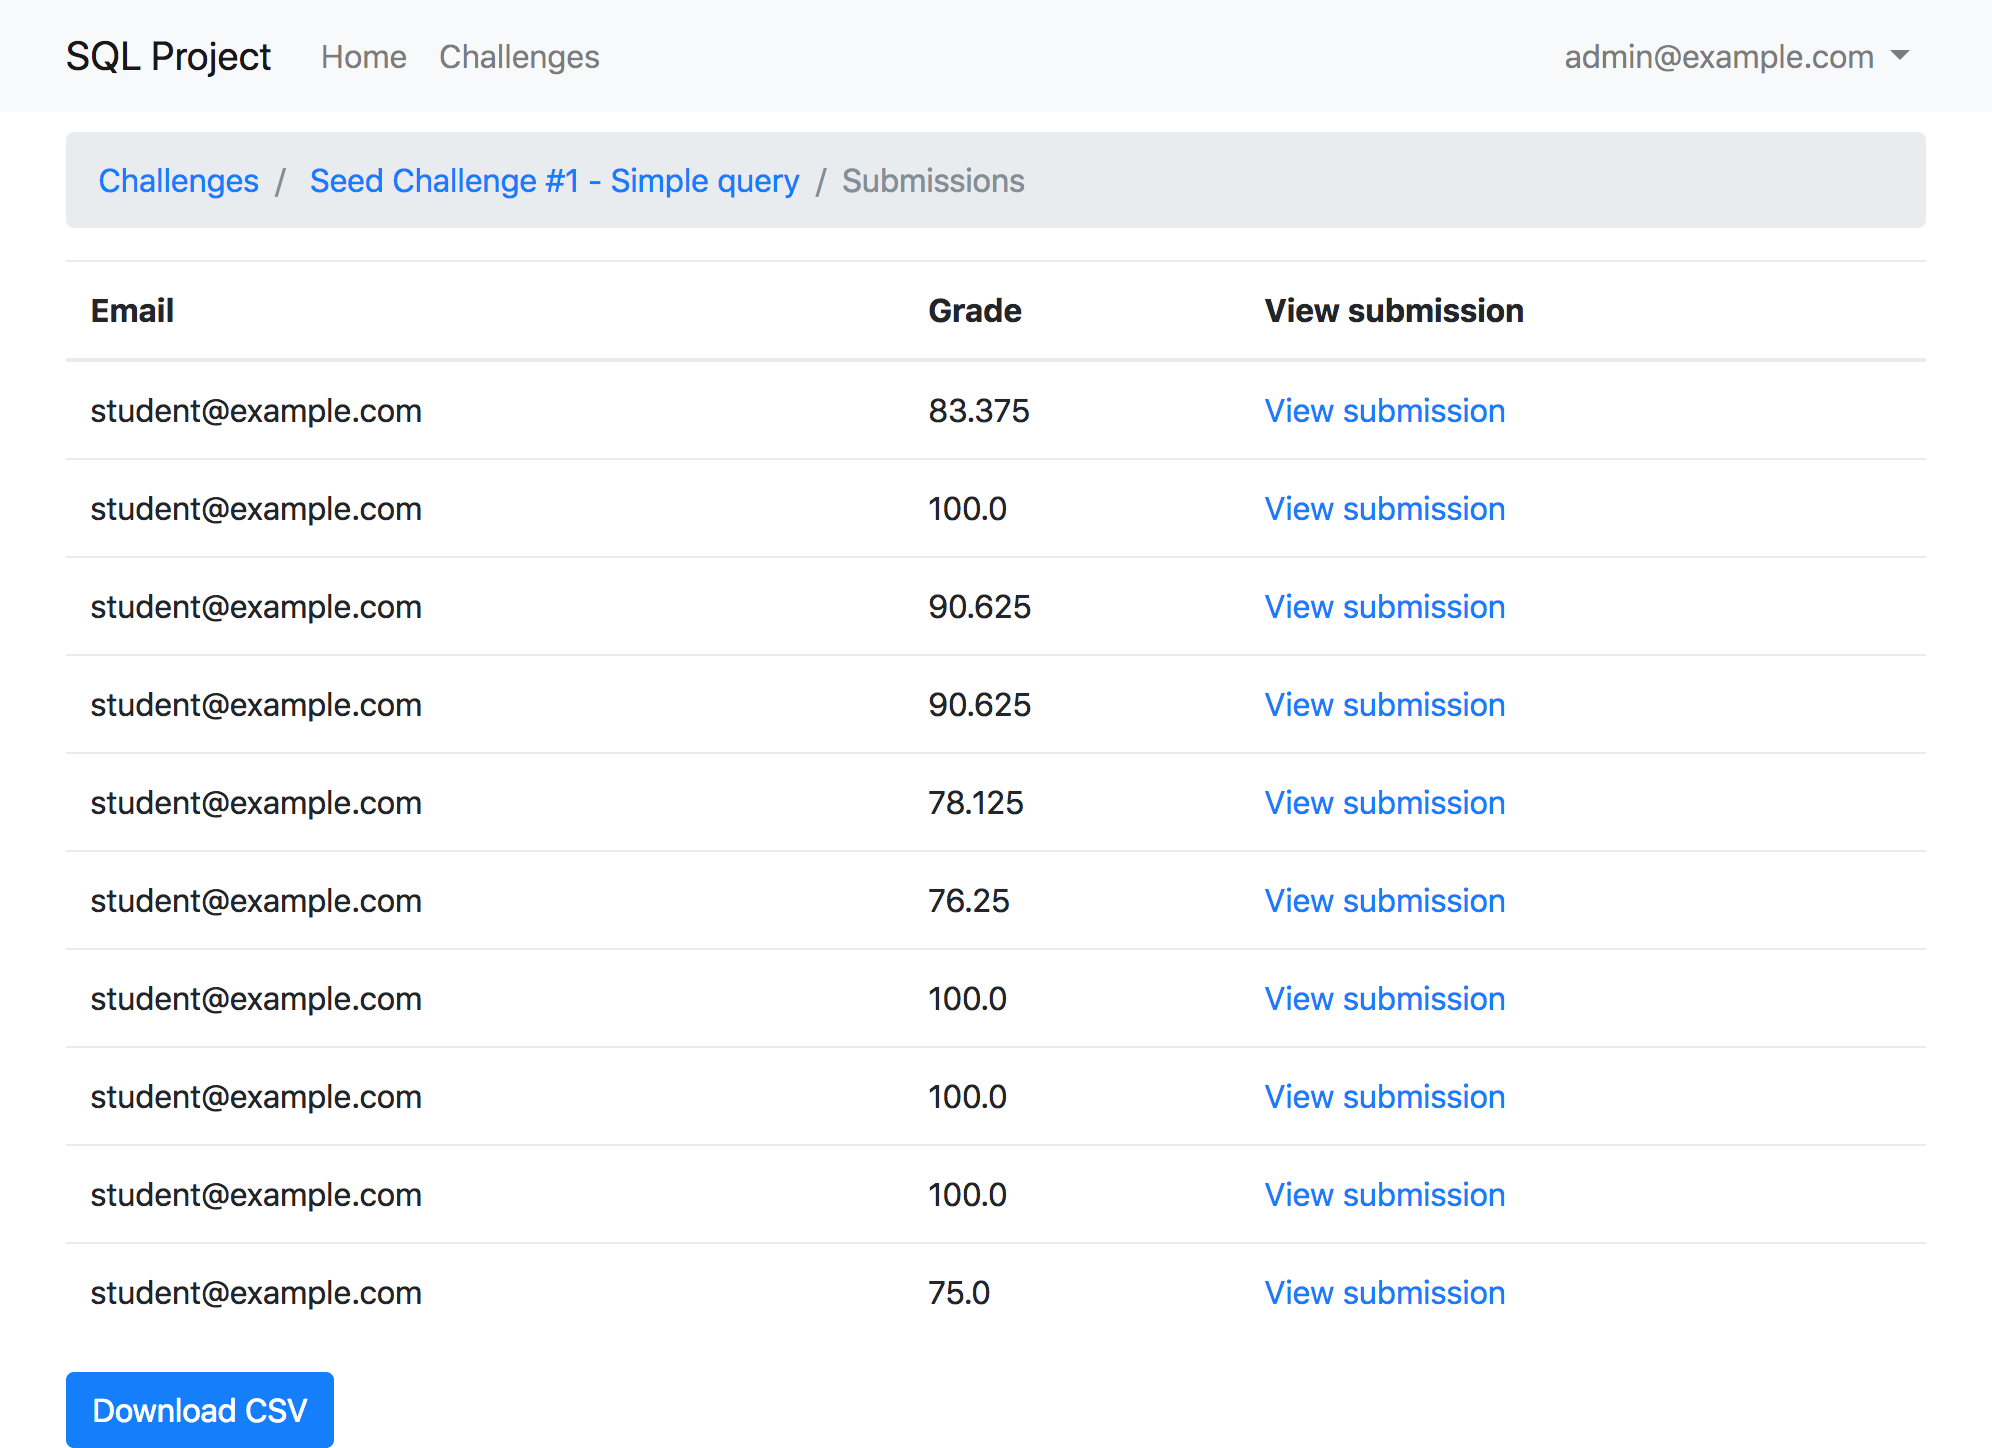
\includegraphics[width=\textwidth/4*3]{Appendices/submissions.png}
    \caption{Submissions for a challenge}
    \label{fig:app:challengeadmin}
\end{figure}

At the bottom of the page there is a Download CSV link that will download a CSV containing the best result for each student.

A instructor can see more details about a submission by clicking the View submission link. The new page will include all details about a submission. An example of such a page is included in figure \ref{fig:app:submission_report}.

\begin{figure}
    \centering
    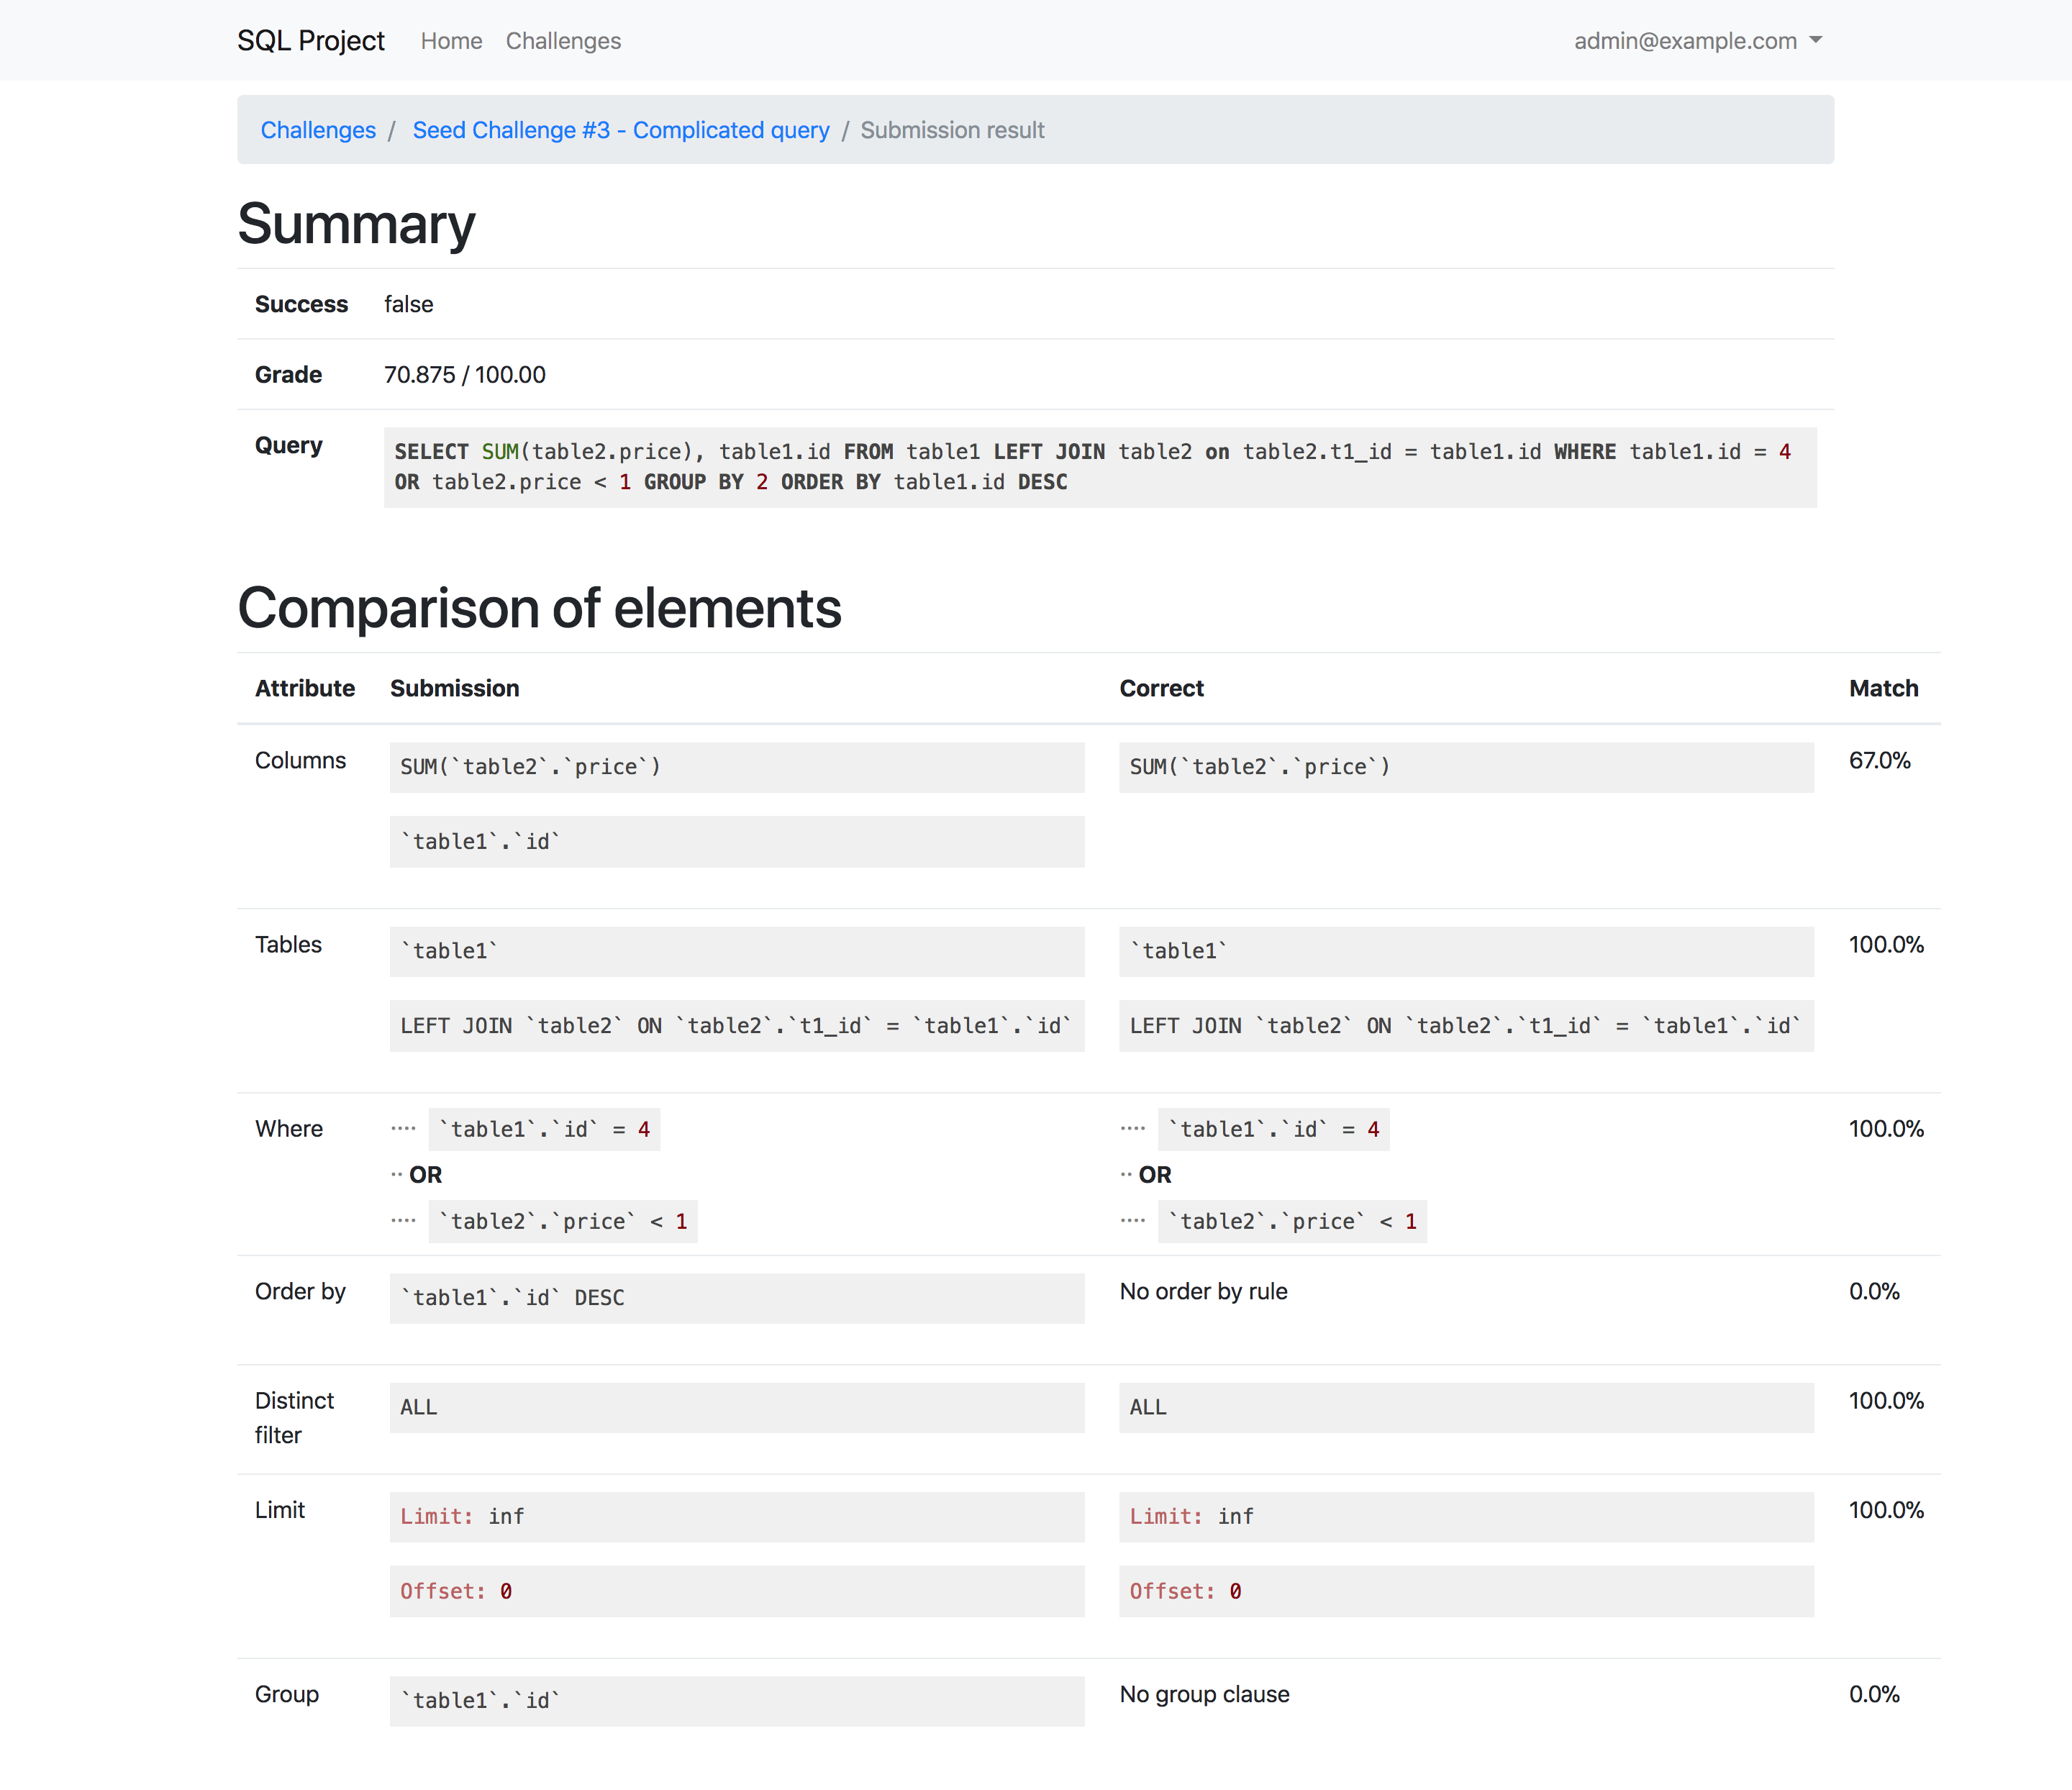
\includegraphics[width=\textwidth/4*3]{Appendices/submission_report.png}
    \caption{Caption}
    \label{fig:app:submission_report}
\end{figure}
% \chapter{Source Code}
\section{Instructions}
Complete source code listings must be submitted as an appendix to the report. The project source codes are usually spread out over several files/units. You should try to help the reader to navigate through your source code by providing a ``table of contents'' (titles of these files/units and one line descriptions). The first page of the program listings folder must contain the following statement certifying the work as your own: ``I verify that I am the sole author of the programs contained in this folder, except where explicitly stated to the contrary''. Your (typed) signature and the date should follow this statement.

All work on programs must stop once the code is submitted to KEATS. You are required to keep safely several copies of this version of the program and you must use one of these copies in the project examination. Your examiners may ask to see the last-modified dates of your program files, and may ask you to demonstrate that the program files you use in the project examination are identical to the program files you have uploaded to KEATS. Any attempt to demonstrate code that is not included in your submitted source listings is an attempt to cheat; any such attempt will be reported to the KCL Misconduct Committee.

\textbf{You may find it easier to firstly generate a PDF of your source code using a text editor and then merge it to the end of your report. There are many free tools available that allow you to merge PDF files.}


\end{document}
